\documentclass{kecsmstr}
\usepackage{etex}
\usepackage{graphicx, epstopdf, amsmath, amssymb, color, caption, subcaption, comment, booktabs, mathabx, mathtools, varwidth, setspace, algorithm, fixltx2e, nicefrac, pgfplots, tikz}
\usetikzlibrary{pgfplots.groupplots}
\usepackage{titletoc}
\usepackage{etoolbox}
\pgfplotsset{compat=1.10}
\usepackage[algo2e, longend, noline, linesnumbered]{algorithm2e}
\usepackage{caption}
\let\cleardoublepage\clearpage
\SetKwIF{If}{ElseIf}{Else}{if}{then}{else if}{else}{endif}
\DeclarePairedDelimiter{\ceil}{\lceil}{\rceil}
\DeclarePairedDelimiter{\floor}{\lfloor}{\rfloor}
\DeclareMathOperator*{\argmax}{arg\,max}
\DontPrintSemicolon
\newcommand{\bE}{\mathbb{E}}
\newcommand{\eg}{{\it e.g.,}~}
\newcommand{\ie}{{\it i.e.,}~}
\newcommand{\cf}{{cf.}~}
\newcommand{\func}[1]{{\sc #1}}
\newcommand{\mctssr}{MCTS_{\mathcal{S}\mathcal{R}}}
\newcommand{\tuple}[1]{\ensuremath{\left \langle #1 \right \rangle }}
\newcommand{\TODO}[1]{\textbf{\color{red}#1}}
\newcommand\mycommfont[1]{\footnotesize\ttfamily{#1}}
\SetCommentSty{mycommfont}

\newcommand{\toexpand}[1]{{\it $\ll$ #1 ... $\gg$ }} 

\newcommand\NoIndent[1]{%
  \par\vbox{\parbox[t]{\linewidth}{#1}}%
}

\graphicspath{{img/}}
\DeclareGraphicsExtensions{.pdf,.jpg,.png,.eps}

\titlecontents{figure}[2.0em]{}{\contentslabel{2.3em}}{}{\titlerule*[0.25pc]{.}\contentspage}{}
\titlecontents{table}[2.0em]{}{\contentslabel{2.3em}}{}{\titlerule*[0.25pc]{.}\contentspage}{}
\contentsuse{algorithm}{loa}
\titlecontents{algorithm}[2.0em]{}{\contentslabel{2.3em}}{}{\titlerule*[0.25pc]{.}\contentspage}{}

\let\listofalgorithms\listoftables
\patchcmd{\listofalgorithms}{\listtablename}{\listalgorithmname}{}{}
\patchcmd{\listofalgorithms}{\listtablename}{\listalgorithmname}{}{}
\patchcmd{\listofalgorithms}{\listtablename}{\listalgorithmname}{}{}
\patchcmd{\listofalgorithms}{lot}{loa}{}{}


\newcommand{\keywords}[1]{\par\addvspace\baselineskip
\noindent\keywordname\enspace\ignorespaces#1}

\title{Novel Selection Methods For Monte-Carlo Tree Search}
\author{Tom Pepels}

\thesistype{Master of Science of Artificial Intelligence}

\thesisdate{2 July 2014} \thesisnumber{14-14}

%Thesiscommittee: use \\ to separate members
\committee{Dr.~Mark~H.M. Winands\\
           Dr.~Marc~Lanctot}
% ================================

\begin{document}

% leave this in place! =============
\makeheaders \pagenumbering{roman} \maketitle \setcounter{page}{2}
\emptypage
% ================

\chapterx{Preface} 
In this thesis I present the result of my investigation into regret minimization for Monte-Carlo Tree Search. The thesis presents the motivation, background, and formal definition of a novel search technique based on minimizing both simple and cumulative regret in a game tree: Hybrid MCTS (H-MCTS). The technique minimizes the two types of regret in a single search-tree. This ensures that recommendations made by the algorithm have a low simple regret, and at the same time internal nodes are sampled efficiently. It was developed for, and tested in six two-player games: Amazons, AtariGo, Ataxx, Breakthrough, NoGo, and Pentalath. The research was performed at the Department of Knowledge Engineering, Maastricht University, The Netherlands.

\vspace{2mm}

Special thanks goes to both Dr. Mark Winands and Dr. Marc Lanctot for providing the inspiration and guidance required to develop this novel algorithm. Their combined experience was crucial to obtain the results presented in this work. Thanks goes to Prof. Dr. Tristan Cazenave for his time and assistance with the implementation of SHOT, and for the experiments he performed in his award-winning engine. Thanks also to Dr. Steve Kroon for his insightful input and assistance in proof-reading the work. Moreover, I would like to thank my wife Priscilla for her support, and for her patience and understanding. Without both her emotional and financial assistance you would not be reading this thesis.
\newline \newline

\vspace{3mm}

\hfill Tom Pepels

\vspace{1mm}

\hfill Maastricht, June 2014
\emptypage

\chapterx{Summary} 
Monte-Carlo Tree Search (MCTS) is a best-first search technique, which bases decisions on sampling the state-space of a domain. In different domains, MCTS has proven to be an effective approach when complex decision-making based on future rewards and outcomes is required. The technique was initially inspired by algorithms used to solve multi-armed bandit (MAB) problems. Such a problem can be described as a single-ply MCTS search, in which an agent is given a choice of options (arms), each with their own probability distribution. Sampling an arm returns a random result from its underlying distribution, and the goal of the agent is to maximize its reward and/or provide a recommendation of which arm has the most rewarding distribution.

\vspace{2mm}

Based on the context of the MAB problem, the agent's goal is to either minimize simple regret, \ie the regret of not recommending the best action, or cumulative regret, \ie regret accumulated over time. Applying this theory to MCTS however, may require more consideration. In a recursive MAB (such as MCTS), where the distribution of each arm is based on an underlying growing search-tree, minimizing a single type of regret throughout the tree implies that at each ply of the tree this specific type of regret minimization is optimal. However, when MCTS is applied to games, the behaviour of the agent in the domain is based solely on its recommendations, \ie the moves it makes in the match, implying that a recommendation made by the algorithm should have an low as possible simple regret.

\vspace{2mm}

The majority of MCTS research uses the UCT selection policy, which minimizes cumulative regret. Other techniques have been proposed to minimize simple regret in MCTS. Based on recent discoveries in simple regret theory in MABs, and two recently introduced MCTS variants, a new MCTS variant is introduced: Hybrid MCTS (H-MCTS). H-MCTS uses different selection policies to specifically minimize both types of regret in different parts of the tree. H-MCTS is inspired by the notion that at the root simple regret is a more natural quantity to minimize. Since all recommendations made by MCTS are based on the values of the root's children, we want the lowest possible simple regret for these nodes. However, deeper down the tree cumulative regret has several beneficial properties which ensure the root's children are properly evaluated. To construct a combination of selection policies, H-MCTS uses SHOT, a recursive version of Sequential Halving, to minimize simple regret near the root, and UCT when the overall budget is lower. 

\vspace{2mm}

A solver is introduced for SHOT and H-MCTS, allowing wins and losses to be proven in the tree. The solver is designed such that it does not disrupt the budget allocations of Sequential Halving, budget that is unspent when a proven node is encountered is spent during later rounds. Finally, an enhancement is introduced for SHOT, which excludes known bad moves from selection. This enhancement ensures that the majority of the allocated budget is spent on promising moves.

\vspace{2mm}

The performance of H-MCTS and the proposed enhancements is assessed in six distinct two-player games: Amazons, AtariGo, Ataxx, Breakthrough, NoGo, and Pentalath. H-MCTS improves performance significantly over UCT in Amazons, AtariGo, Ataxx, and Pentalath when random play-outs are used. Moreover, in Breakthrough H-MCTS outperforms UCT when using an informed play-out policy. \emptypage

\tableofcontents \clearpage
\listofalgorithms
\listoffigures \clearpage
\listoftables
\pagenumbering{arabic}

% --------------------------------------------------------------------
% ------------------- ::::::: Introduction ::::::: -------------------
% --------------------------------------------------------------------
\chapter{Introduction}
\label{chap:intro}
\begin{chaptercontents} An overview of Monte-Carlo Tree Search and the main topic of this thesis, simple regret minimization applied to Monte-Carlo Tree Search. Moreover, the problem statement and research questions are drafted and a general outline of the structure of the thesis is given.
\end{chaptercontents}

\section{Artificial Intelligence and Games}
Decision-making and problem solving have been core topics in Artificial Intelligence (AI) since its birth over half a century ago. In many domains an agent is required to find a specific sequence of actions to achieve a certain goal. A search algorithm can be used to explore the state space to find rewarding states in the future and determine the best action given the current state.
Given that most real domains are too complicated to result in a limited, specific set of rules for the agent to follow, an abstract domain is more appropriate when investigating search algorithms. For a single agent, puzzles, graph problems and simplified real-world models are often investigated. In this case, the agent's goals are non-adversarial, and it takes to maximize its utility over time to reach a set goal. When more than one agent is involved, games provide adversarial challenges with simple rules that result in large and complex state spaces. For most interesting games, an exhaustive search is not feasible, but heuristics and approximation techniques have been developed.

Even before the first computer capable of playing games at a reasonable level was developed, Alan Turing was thinking about computer chess~\citebay{turing1988chess}. Over the decades, faster computers allowed for deeper investigation into game-playing algorithms such as $\alpha\beta$~\citebay{knuth1976analysis}, Principal-Variation Search~\citebay{marsland1983relative}, Proof-number search~\citebay{allis1994proof}. One of the reasons game AI research has sparked interest over the years is that its techniques can be directly measured against human players. In 1997, {\sc Deep Blue}~\citebay{campbell2002deep} defeated then-reigning world chess champion Garry Kasparov in a six-game match, the first time a computer beat the human champion. After plentiful research had been performed in computer chess, Go was the next target for game AI research. In contrary to chess, for Go it is not straightforward to find a decent evaluation function. Moreover, in Go, over the course of the game stones can be played anywhere on the board leading to a high branching factor.

With the introduction of Monte-Carlo Tree Search~\citebay{kocsis2006bandit,coulom2007efficient}, and UCT~\citebay{kocsis2006bandit}, researchers could reach expert-level play in Go~\citebay{gelly2008achieving,lee2010current} on small boards. Since it requires no static heuristic evaluation, using simulations to determine the rewards of states in the tree, and a selection policy to explore the tree, MCTS performed better than any algorithm had before~\citebay{lee2009computational}. The success of MCTS and UCT in Go sparked researchers' interests in developing a better understanding of the algorithm and applying it to different domains ranging from games, planning problems and real-time domains~(\cf~\citeay{browne2012survey}).
\newpage
\section{Monte-Carlo Tree Search}
Monte-Carlo Tree Search (MCTS) is a best-first search method based on random sampling by Monte-Carlo simulations of the state space for a specified domain~\citebay{coulom2007efficient,kocsis2006bandit}. In gameplay, this means that decisions are made based on the results of randomly simulated play-outs. MCTS has been successfully applied to various turn-based games such as Go~\citebay{gelly2008achieving,lee2010current}, Lines of Action~\citebay{Winands2010b}, and Hex~\citebay{arneson2010monte}. Moreover, MCTS has been used for agents playing real-time games such as the Physical Traveling Salesman~\citebay{powleytsp}, and Ms~Pac-Man~\citebay{realtime2014}, and real-time strategy games~\citebay{balla2009uct}, but also in real-life domains such as optimization, scheduling, and security~\citebay{browne2012survey}.

\begin{figure}[ht]
	\centering
	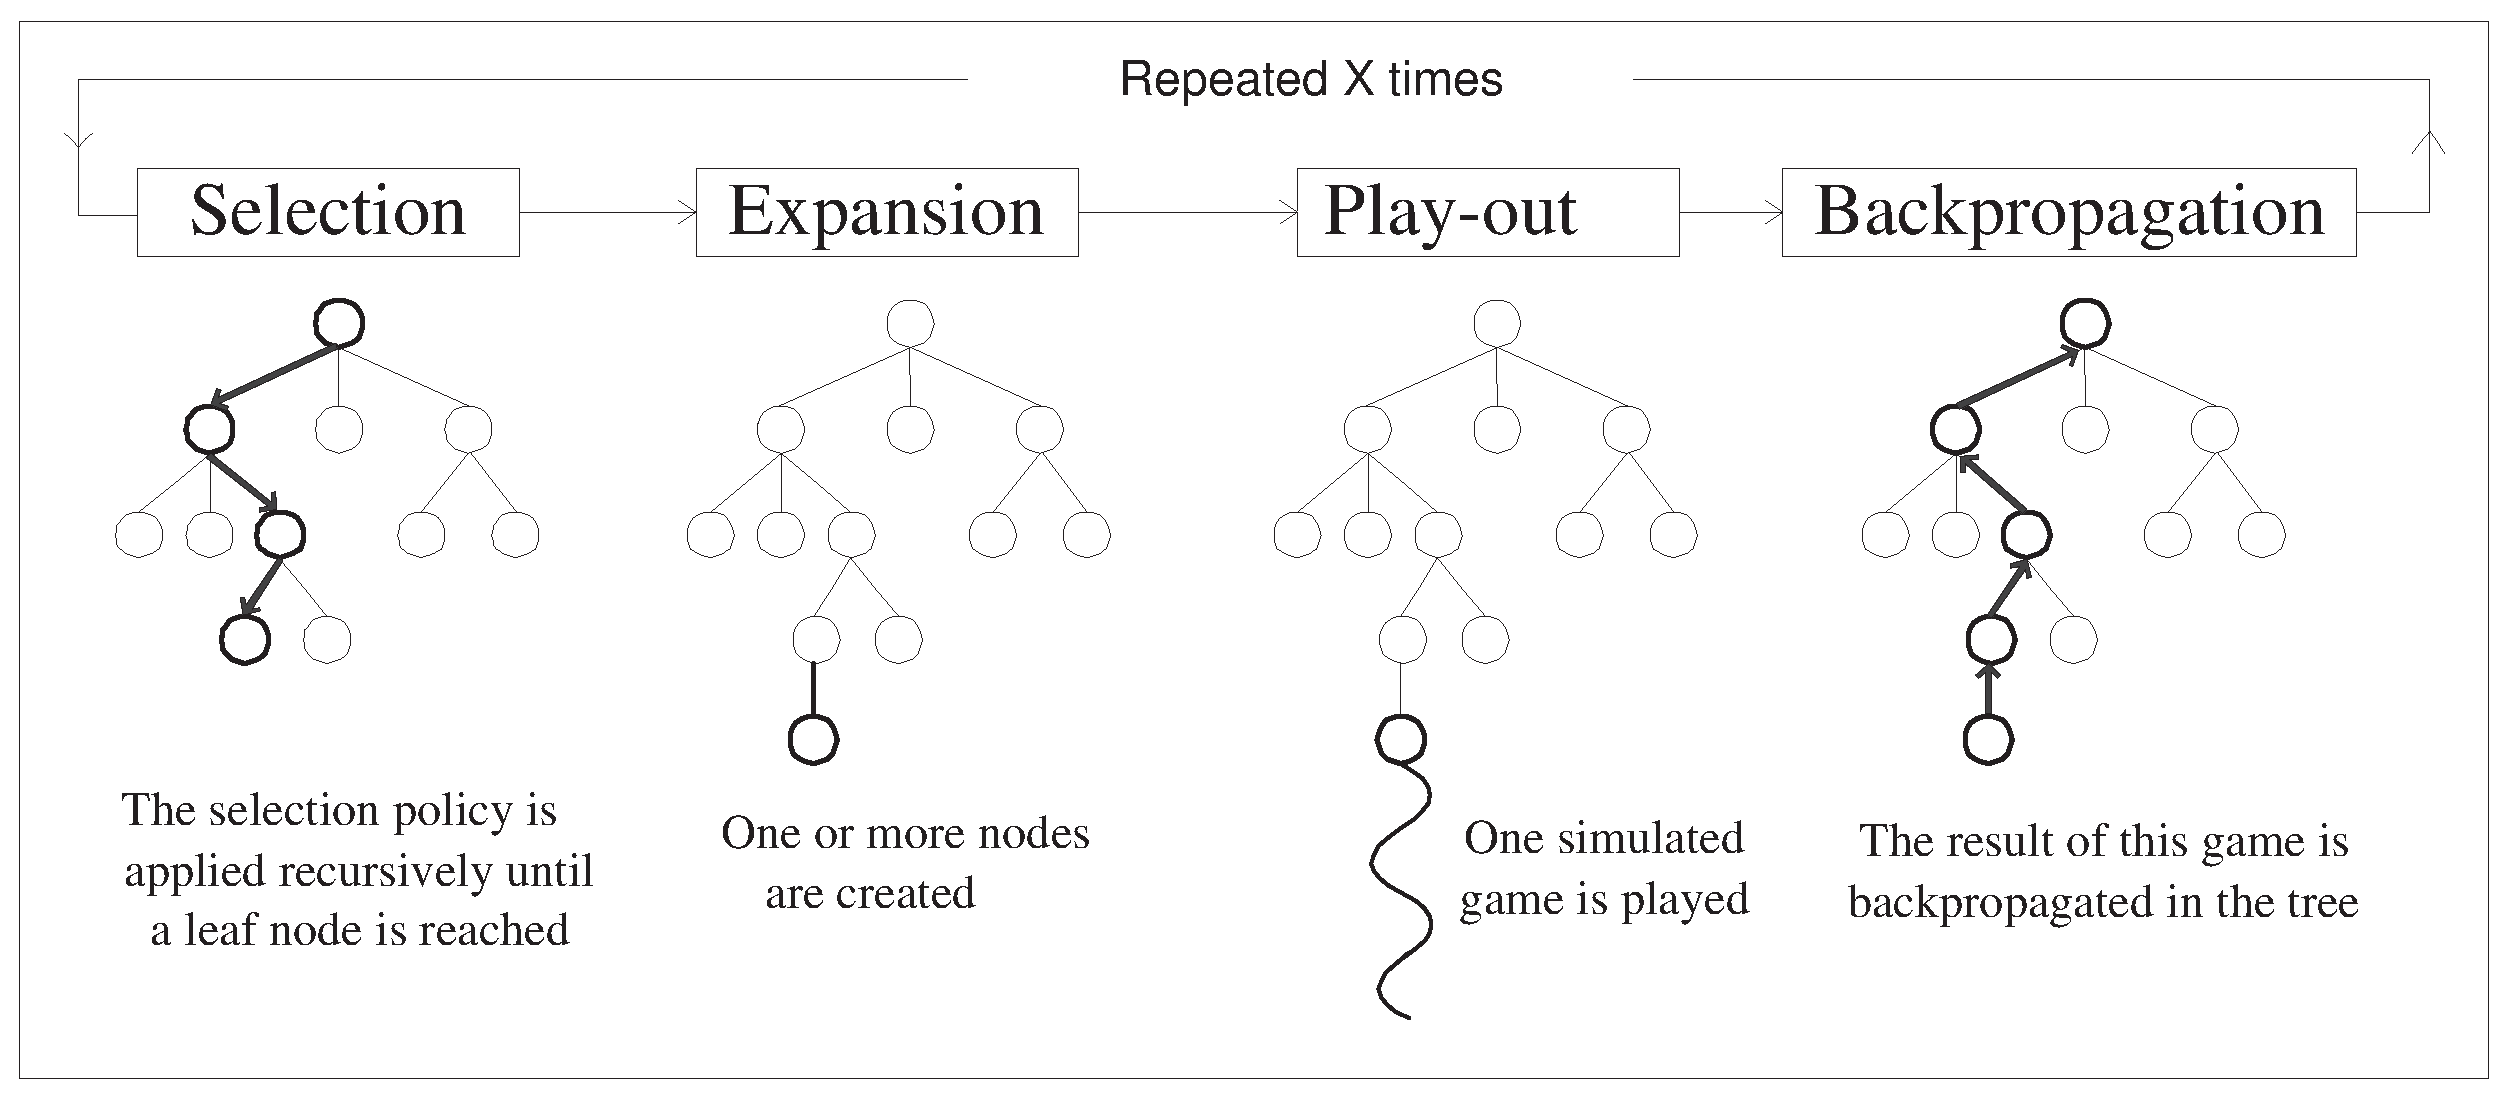
\includegraphics[width=.9\textwidth]{img/figure1.eps}
	\caption[Strategic steps of Monte-Carlo Tree Search.]{Strategic steps of Monte-Carlo Tree Search~\protect\citebay{chaslot2008progressive}.}
	\label{fig:mcts-algorithm}
\end{figure}
\noindent In MCTS, a tree is built incrementally over time, which maintains statistics at each node corresponding to the rewards collected at those nodes and number of times  they have been visited. The root of this tree corresponds to the current position. When using a bandit-based method to select moves, such as in UCT, MCTS resembles a recursive multi-armed bandit. The basic version of MCTS consists of four steps, which are performed iteratively until a computational threshold is reached, \ie a set number of iterations, an upper limit on memory usage, or a time constraint. The basic version of MCTS consists of four steps \citebay{chaslot2008progressive}:
\begin{itemize}
\item {\bf Selection}. Starting at the root node, children are selected recursively according to a selection policy. When a leaf node is reached that does not represent a terminal state it is selected for expansion.
\item {\bf Expansion}. One or more children are added to the selected leaf node.
\item {\bf Play-out}. A simulated play-out is performed, starting from the state of (one of) the added node(s). Moves are performed randomly or according to a heuristic strategy until a terminal state is reached.
\item {\bf Back-propagation}. The result of the simulated play-out is propagated immediately from the added node back up to the root node. Statistics are updated along the tree for each node selected during the selection phase and visit counts are increased.
\end{itemize}
The combination of moves selected during the selection step, and the play-out form a single simulation. During the selection step, moves are executed according to the nodes selected in the tree, and during play-out moves are performed randomly, or according to some play-out policy.

Because results are immediately back-propagated, MCTS can be terminated any time to determine the decision to be made. Moreover, no static heuristic evaluation is required when simulations reach an end state. However, in most cases it is beneficial to add domain knowledge for choosing moves made during the play-out.

The main benefit of MCTS is that it requires no explicit heuristic state evaluation. Rather, states are evaluated by repeatedly sampling them and measuring an average reward. It is often beneficial to add some domain knowledge to the play-outs such that the simulated games better approximate good play. Moreover, many enhancements to MCTS have been proposed to improve the general performance of the algorithm. Some of the most notable enhancements are: MCTS-Solver \citebay{Winands2008}, which recognizes solved wins and losses in the tree and back-propagates their values, and RAVE~\citebay{gelly2007}, used to speed up node valuation in the tree. Moreover, several on-line learning techniques for play-out policies have been proposed, such as low-level $\alpha\beta$ searches~\citebay{Winands2011}, the Last-Good-Reply policy~\citebay{baier2010power}, Move-average Sampling Technique (MAST)~\citebay{finnsson2008simulation}, and N-grams~\citebay{Tak2012}. Combining these enhancements often offers greatly improved play by MCTS.

\section{Regret Minimization}
Algorithms used in multi-armed bandit research have been developed to minimize \emph{cumulative regret}. Cumulative regret is the expected regret of not having sampled the optimal decision. This type of regret is accumulated during execution of the algorithm, each time a non-optimal arm is sampled the cumulative regret increases. UCB1~\citebay{auer2002using} is a selection policy for the MAB problem, which minimizes cumulative regret at a fast rate, converging to the empirically best arm fast. Once a candidate best arm is found by exploring the available options, UCB1 exploits it by repeated sampling. This policy was adapted to be used in MCTS in the form of UCT~\citebay{kocsis2006bandit}.

Recently, \emph{simple regret} has been proposed as a new criterion for assessing the performance of both MAB~\citebay{audibert2010best,Bubeck11Pure} and MCTS~\citebay{tolpin2012mcts,Feldman12BRUE} algorithms. Simple regret is defined as the expected error between an algorithm's recommendation and the optimal decision. Simple regret is a naturally fitting quantity to optimize in the MCTS setting, since all simulations executed by MCTS are for the mere purpose of learning good moves. However, the final move chosen after all simulations are performed, \ie the \emph{recommendation}, is the one that has real consequence. Therefore, the choice of this move should have as low as possible simple regret. Moreover, once MCTS finds a good move with high certainty, the utility of re-selecting that move diminishes over time. When a promising node, or group of nodes is visited too often, at a certain point insufficient simulation time remains to determine whether there exists a viable alternative. Rather it may be favourable to explore other options sooner, even if a single move is identified as the best. At the same time, MCTS should not `waste' its time on moves that are expected to be bad.

This is the driving idea behind pure exploration algorithms such as Successive Rejects~\citebay{audibert2010best} and Sequential Halving~\citebay{Karnin13SH}. Contrary to UCB, these algorithms have no specific exploitation phase, they divide their time uniformly between a continuously reduced set of options. The final recommendation is the single arm that remains after all trials are finished. These pure exploration techniques form the basis of the simple regret argument for MCTS presented in this thesis.
\newpage
\section{Problem Statement and Research Questions}
When MCTS is applied to games it is only the final recommendation, \ie the actual move played, that has an impact. To this end, we want the probability of selecting a suboptimal move, \ie the expected simple regret, to be as low as possible. Based on this assumption, simple regret minimization can be a better way to determine a move's utility. As such, a method that minimizes both types of regret in their appropriate settings can improve the overall performance of MCTS. Simple regret optimization (pure exploration) has practical problems, especially at low search times because it spends more time on suboptimal options, whereas techniques based on cumulative regret minimization perform particularly well under such limited circumstances. Currently, several algorithms have been proposed to minimize simple regret. However, some do not improve performance in games, while others only provide benefits in specific circumstances.

The problem statement of the thesis is:
\newline \newline
\emph{How can a Monte-Carlo Tree Search variant be constructed to minimize both simple and cumulative regret effectively?}
\newline \newline
The following four research questions arise from this problem statement:
\begin{enumerate}

\item{\emph{How can a search technique minimize both simple, and cumulative regret in a game tree?}}
\item{\emph{When should selection switch from simple to cumulative regret minimization in the tree?}}
\newline
\NoIndent{To answer these questions, an investigation into state-of-the-art multi-armed bandit algorithms is performed. Two MCTS variants that minimize simple regret, SHOT~\citebay{Cazenave14SHOT} and the SR+CR scheme~\citebay{tolpin2012mcts} are discussed. These algorithms provide the inspiration and technique for a new Hybrid MCTS (H-MCTS).
Given the new Hybrid technique, the initial assumption regarding simple regret minimization in games ought to be verified:}

\item{\emph{Do pure exploration selection policies in H-MCTS improve performance in two-player games?}}
\newline
\NoIndent{This question is answered by performing experiments in six distinct two-player games: Amazons, AtariGo, Ataxx, Breakthrough, NoGo, and Pentalath. The performance of H-MCTS' is compared to both UCT and SHOT in these games.}

\NoIndent{The last research question relates to an existing MCTS enhancement called MCTS-Solver~\citebay{Winands2008}, which back-propagates proven wins and losses in the game tree:}

\item{\emph{How can the MCTS-Solver be adapted to work with H-MCTS and SHOT?}}
\newline
\NoIndent{To address the last research question, the MCTS-Solver is adapted and implemented in SHOT and H-MCTS. }
\end{enumerate}

\section{Thesis Outline}

The thesis opens with two introductory chapters introducing and discussing the background of the theory used. \textbf{Chapter \ref{chap:mab}}, which discusses the Multi-armed Bandit problem and its application to MCTS, and \textbf{Chapter \ref{chap:mctssr}}, in which current simple regret minimizing MCTS algorithms are discussed. The former details the exact difference between simple and cumulative regret, and how these types of regret may be minimized using different selection policies, and the latter shows how these selection policies are applied to MCTS.

Next, \textbf{Chapter \ref{chap:hybmcts}} goes into detail on H-MCTS. Based on the analysis in the previous chapters, the new algorithm is defined and described. Moreover, the problems and shortcomings of the algorithm are discussed, and possible solutions provided. In \textbf{Chapter \ref{chap:experiments}} the proposed algorithm is tested on six two-player games: Amazons, AtariGo, Ataxx, Breakthrough, NoGo, and Pentalath. \textbf{Chapter \ref{chap:conclusion}} concludes the thesis, and offers directions for future research and improvements.

% --------------------------------------------------------------------------------------
% ------------------- ::::::: Regret And Multi-Armed Bandits ::::::: -------------------
% --------------------------------------------------------------------------------------
\chapter{Regret and Multi-Armed Bandits}
\label{chap:mab}
\begin{chaptercontents} The foundation of regret minimization for Monte-Carlo Tree Search (MCTS) is given. Given that UCT is defined as a recursive multi-armed bandit (MAB) algorithm, regret minimization is discussed in this context first. Two algorithms designed to minimize simple regret in MABs are outlined. Moreover, the link between simple and cumulative regret is detailed and recent findings are discussed. 
\end{chaptercontents}

\section{Introduction}
The multi-armed bandit (MAB) problem is defined as a stochastic decision-making problem~\citebay{Robbins_someaspects}. An agent is faced with several options, each with their own reward distribution. Based on sampling the search space an agent is to select the option with the best reward distribution. Generally the problem is described as choosing between the most rewarding arm of a multi-armed slot machine found in casinos. The agent can explore by pulling an arm and observing the resulting reward. The reward is drawn from a fixed probability distribution. Each pull and the returned reward constitutes a sample. When combined with MCTS, the MAB problem becomes both recursive and non-stationary which is explained in Chapter~\ref{chap:mctssr}.

In the classic MAB setting, the goal is to maximize the cumulative sum of rewards, \eg winning the most money in the slot machine example. Since the agent does not know the distribution of the arms beforehand, he has to \emph{explore} the possible choices, and when a rewarding arm is found, \emph{exploit} this option to gain a high total reward. Generally, after a certain limit, \eg a time-span or number of trials, the agent must return a recommendation to determine the best arm.

The performance of the agent can be evaluated by observing the difference in the rewards obtained over time and the theoretical reward obtained by pulling only the true best arm, called \emph{cumulative regret}. Or, in the case of \emph{simple regret}, observing the difference between the recommended arm and the true best arm, after the forecaster makes its final recommendation.
\vspace{2 mm}

In this chapter the different facets of the MAB problem are discussed and related to MCTS. In Section \ref{sec:mabprob} a formal definition of the two types of regret is given. Next, Section \ref{sec:ucb} discusses the well-known UCB1 selection policy and its relation to MCTS. This is followed by a review of two recently introduced selection policies for MAB aimed at minimizing simple regret, in Section \ref{sec:pureexplmab}.

\section{Regret and The Multi-Armed Bandit Problem}
\label{sec:mabprob}
Suppose a trial is set-up such that a forecaster (a player, or agent) has $K$ actions, which can be repeatedly sampled over $n \in \{ 1, 2, \cdots, T \}$ trials. Each arm has a mean reward $\mu_i$, and there exists an maximum mean reward $\mu^*$. Suppose further that the forecaster employs a selection policy $I(n)$ that outputs some $a$ to be sampled at time $n$, and a recommendation policy $J(n)$ that selects the best arm at time $T$.

\emph{Cumulative regret} is defined as the regret of having not sampled the best single action in hindsight, 
\begin{equation}
R_n = \sum_{t = 1}^{n}{\mu^* - \mu_{I(t)}}.
\end{equation}
In other words, the regret is accumulated over time, for each sample the forecaster takes.

Now suppose that we change the experimental set-up, such that the actions chosen on trials $1, 2, \ldots, T-1$ are taken under some realistic ``simulated environment'' that represents the true on-line decision problem but without committing to the actions. The only \emph{real} decision is made at step $T$ after having played $T-1$ simulations. In contrast, \emph{simple regret}~\citebay{Bubeck11Pure} quantifies only the regret for the recommendation policy $J$ at time $T$,

\begin{equation}
r_n = \mu^* - \mu_{J(n)},
\end{equation}
\ie the regret of not having recommended the best action.

Given these definitions, a performance metric for a selection technique can be described as the expected cumulative $\bE R_n$ or simple regret $\bE r_n$ over different experiments. In their analysis of the links between simple and cumulative regret,~\citeaby{Bubeck11Pure} found that upper bounds on $\bE R_n$ lead to lower bounds on $\bE r_n$, and that the smaller the upper bound on $\bE R_n$, the higher the lower bound on $\bE r_n$, regardless of the recommendation policy, \ie the smaller the cumulative regret, the larger the simple regret. As such, no policy can give an optimal guarantee on both simple and cumulative regret at the same time. In the case of an MAB the strategy used depends on the context of the problem.

\section{Upper Confidence Bounds}
\label{sec:ucb}

\citeaby{auer2002using} proposed a finite time strategy for the MAB problem. Upper Confidence Bounds (UCB) optimizes cumulative regret over time at an optimal logarithmic rate, without knowledge of the reward distributions. The selection policy consists of two terms, 1) the current average reward, and 2) the size of the one-sided confidence interval for the average reward. For each arm, UCB1 gives an upper bounding value, below which, the true expected reward of the arm falls with high probability. The UCB1 selection policy is outlined in Algorithm \ref{alg:ucb}.

\IncMargin{1em}
\RestyleAlgo{boxruled}
\begin{algorithm2e}[ht]
	\Indm
	\KwIn{total budget $T$, $K$ arms}
	\KwOut{recommendation $J_T$}
	\vspace{0.2cm}
	\Indp

	play each arm once, for each arm $i$, update $\bar{x}_i$ with the obtained reward, and $n_i \gets 1$\;

	\For{t=1 \emph{\KwTo} $T$} {
		Sample arm $i$ that maximizes $\bar{x}_i + \displaystyle\sqrt{\frac{2\ln{t}}{n_i}}$ \newline
		$\bar{x}_i$ is the current average reward of arm $i$, $n_i$ is the total number of samples for arm $i$ \;
	}

	\KwRet{the arm with the highest average reward}
  \caption[Upper Confidence Bounds (UCB1)]{Upper Confidence Bounds (UCB1)~\protect\citebay{auer2002using}. \label{alg:ucb}}
\end{algorithm2e}
\DecMargin{1em}

The rate of growth of cumulative regret of UCB1 is $O(\ln(n))$, where $n$ is the number of samples, which was shown to be the optimal rate by~\citebay{lai1985asymptotically}. \citeaby{Bubeck11Pure} show that a recommendation based on such a selection policy suffers a simple regret that decreases at best at a polynomial rate. 

Later in this chapter, in Section \ref{sec:mabmcts} UCB1 is discussed in the context of MCTS. In MCTS, a version of UCB1 adapted to tree search named Upper Confidence Bounds for Trees (UCT) is widely used as the preferred selection policy.

\section{Pure Exploration in Multi-Armed Bandits}
\label{sec:pureexplmab}
Non-exploiting selection policies have been proposed to decrease simple regret at a high rate, and with low bounds. Given that UCB1 has an optimal rate of cumulative regret convergence, and the conflicting limits on the bounds on the regret types shown by~\citeaby{Bubeck11Pure}, policies that have a higher rate of exploration than UCB1 have better bounds on simple regret. 

Consider a uniform selection policy that samples each arm of an MAB $T/K$ times. Assuming that there are $h$ best arms, $(K-h)T/K$ trials are spent sampling inferior arms, and $hT/K$ on the best one(s). Such a selection policy has simple regret $\bE r_n = \bE R_n/n$~\citebay{Bubeck11Pure}.
In games, there are often only a few promising moves to be identified, and therefore when using uniform selection, most time is spent sampling suboptimal arms. Therefore, a more efficient policy is required to ensure that inferior arms are not selected as often as arms with a high utility over time. Two algorithms, discussed in this section, have been proposed to solve this problem.

Both algorithms have shown to outperform the other in different problem settings~\citebay{Karnin13SH}. Sequential Halving gives better results when there are multiple groups of suboptimal arms, or when the arm's rewards form an arithmetic or geometric series. Successive Rejects performs best when there is a single group of suboptimal arms, or when selecting over a small subset of arms. Both methods have proven theoretical guarantees with regard to the simple regret bounds, and a near-optimal, exponential rate of decrease on simple regret. Based on this it holds merit to consider these algorithms as candidate substitutes for UCT in MCTS. However, based on the analysis made by~\citebay{Bubeck11Pure} discussed in Section \ref{sec:mabprob}, any method that effectively minimizes simple regret has inferior bounds on its cumulative regret. Therefore, there may be some trade-off between using pure exploration methods and UCT.

\subsection{Successive Rejects}
\IncMargin{1em}
\RestyleAlgo{boxruled}
\begin{algorithm2e}[ht]
	\Indm
	\KwIn{total budget $T$, $K$ arms}
	\KwOut{recommendation $J_T$}
	\vspace{0.2cm}
	\Indp
	$S_1 \gets \{1,\dots,K\}$, $n_0 \gets 0$										\; 
	$\widebar{log}(K) \gets \frac{1}{2} + \sum_{i=2}^{K} \frac{1}{i}$				\;
	\BlankLine
	\ForEach{$k\in\{1,\dots,K-1\}$} {
		$n_k = \displaystyle\ceil[\bigg]{\frac{1}{\widebar{log}(K)} \frac{T-K}{K+1-k}}$				\;
	}
	\BlankLine
	\For{k=1 \emph{\KwTo} $K-1$}{
		Sample each arm $i\in S_k$ $n_k - n_{k-1}$ times 						\;	\label{succrej:subtr}
		update the average reward of each arm based on the samples 		\;
		$S_{k+1} \gets$ the $|S_k|-1$ empirically best arms from $S_k$			\;
	}
	\BlankLine
	\KwRet{the single element of $S_K$}
  \caption[Successive Rejects]{Successive Rejects~\protect\citebay{audibert2010best}. \label{alg:succrej}}
\end{algorithm2e}
\DecMargin{1em}

Successive Rejects~\citebay{audibert2010best} works by successively removing the single worst arm from the selection. The algorithm computes a budget $n_k$ for each round. During a round, each arm is selected uniformly, and after each round, the empirically worst arm is removed from the selection and the next round starts. The current average values of the arms are retained between rounds. The lengths of the rounds are computed in such a manner that a specific lower bound on simple regret is guaranteed.

Successive Rejects is detailed in Algorithm~\ref{alg:succrej}. Because $n_0 = 0$, the algorithm starts with a relatively long initial round, followed by the shortest one, due to the subtraction on line \ref{succrej:subtr}. However, the length of the rounds increases when more arms are removed. An example run is depicted in Figure~\ref{fig:succ-rej}, where a total budget $T = 200$ is allocated to 5 arms, the number of samples per arm for each round is shown. For the first round the trials per arm are $\ceil{\frac{60}{107} \frac{200-5}{5+1-1}} - 0 = 22$ subsequently, for the second round $\ceil{\frac{60}{107} \frac{200-5}{5+1-2}} - 22 = 6$ and so on. The recommended arm is sampled a total of $57$ times.

\begin{figure}[ht]
	\centering
	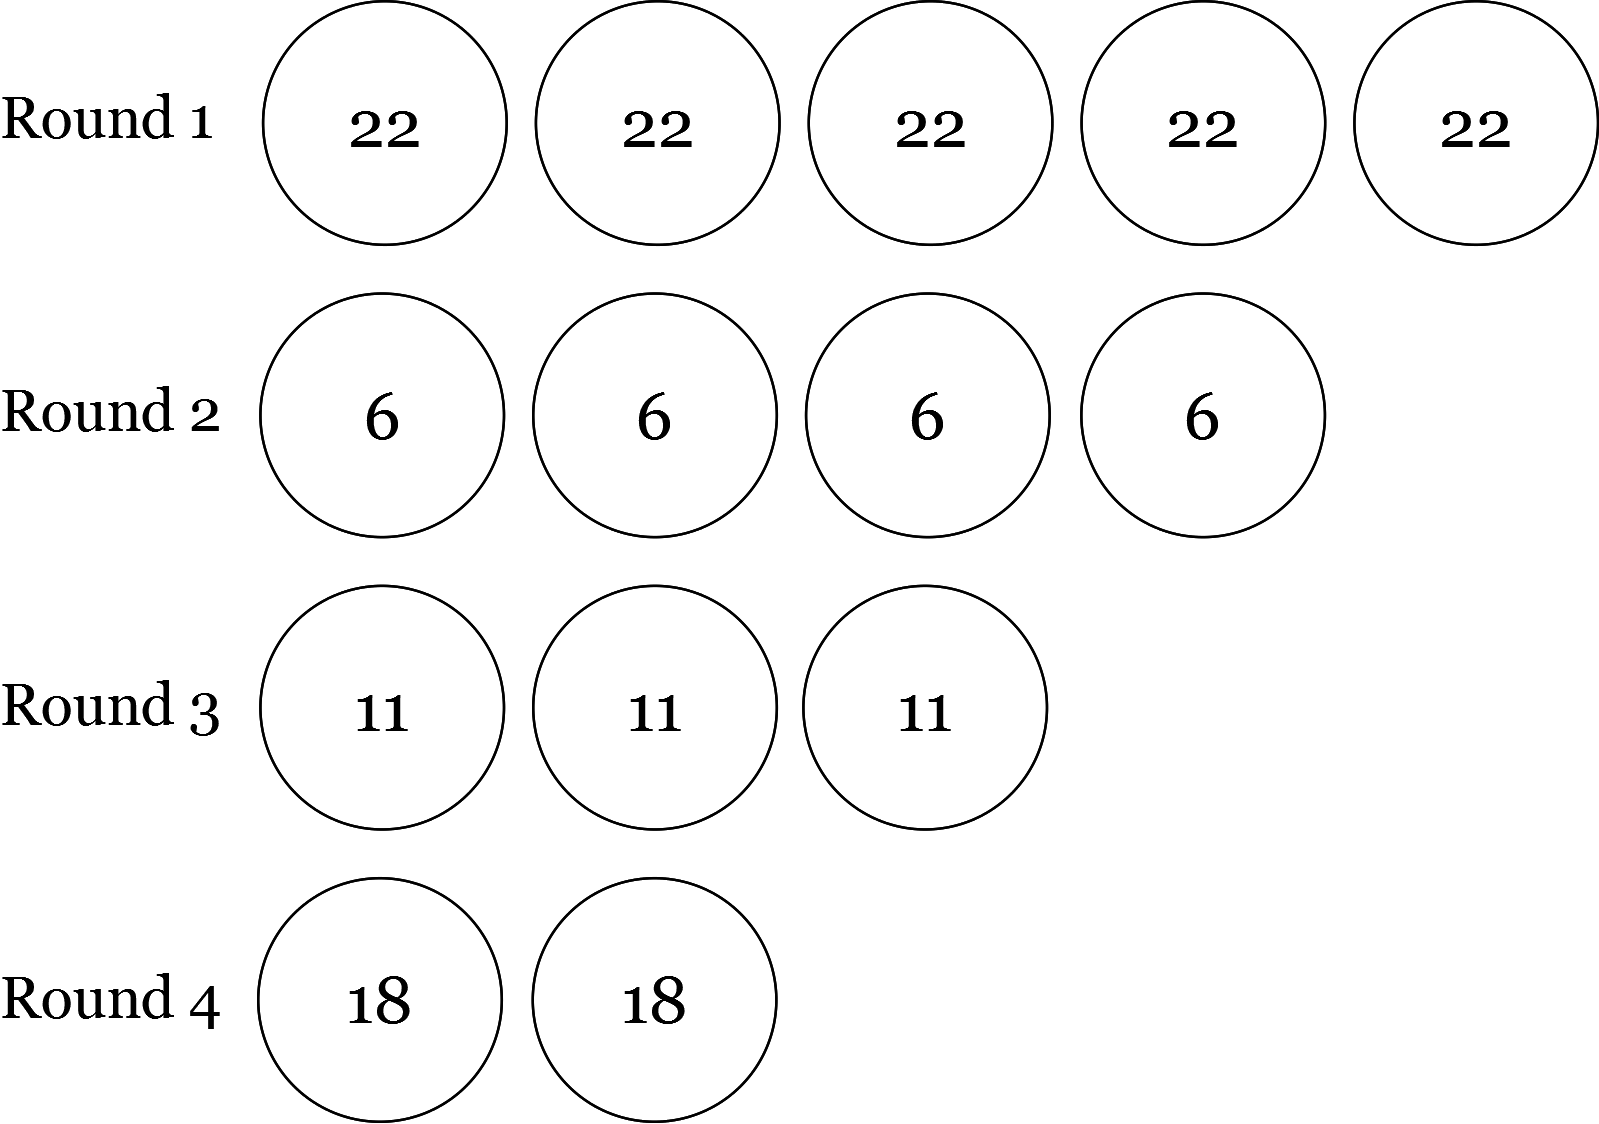
\includegraphics[width=.6\textwidth]{img/succ_rej.png}
	\caption[Successive Rejects example]{Successive Rejects example on 5 arms and a total budget of 200.}
	\label{fig:succ-rej}
\end{figure}

\newpage

\subsection{Sequential Halving}
Sequential Halving~\citebay{Karnin13SH} takes an approach similar to Successive Rejects. As with Successive Rejects, search time is divided into rounds, and during each round arms are sampled uniformly. However, instead of removing a single arm from selection after each round, half the arms are removed until a single one remains. The rounds in Sequential Halving are equally distributed such that constitute the same number of trials, but with a decreased subset of arms to select. Sequential Halving is detailed in Algorithm~\ref{alg:seqhalv}.

\IncMargin{1em}
\begin{algorithm2e}[ht]
\setstretch{1.1}
	\KwIn{total budget $T$, $K$ arms}
	\KwOut{recommendation $J_T$}
	\vspace{0.1cm}
	$S_0 \gets \{1,\dots,K\}$,
	$B \gets \ceil{\log_2{K}} - 1$														\;
	\BlankLine
	\For{k=0 \emph{\KwTo} $B$}{
		sample each arm $i \in S_k$, 										
		$n_k = \floor[\bigg]{\frac{T}{|S_k|\ceil{\log_2{|S|}}}}$
		times 																				\;
		\vspace{0.1cm}
		update the average reward of each arm based on the rewards 		\;
		$S_{k+1} \gets$ the $\ceil{|S_k|/2}$ arms from $S_k$ with the best average			\;
	}
	\KwRet{the single element of $S_B$}
  \caption[Sequential Halving]{Sequential Halving~\protect\citebay{Karnin13SH}. \label{alg:seqhalv}}
\end{algorithm2e}
\DecMargin{1em}

An example of the budget allocation by Sequential Halving is depicted in Figure \ref{fig:seq-halving}, where a total budget $T = 200$ is allocated to $5$ arms, the allocated budget per arm for each round is shown. At time $T$, after $\ceil{\log_2{5}}=3$ rounds, the single remaining arm is recommended. This arm is sampled $68$ times, $11$ times more than the recommended arm in the same example given for Successive Rejects.

\begin{figure}[ht]
	\centering
	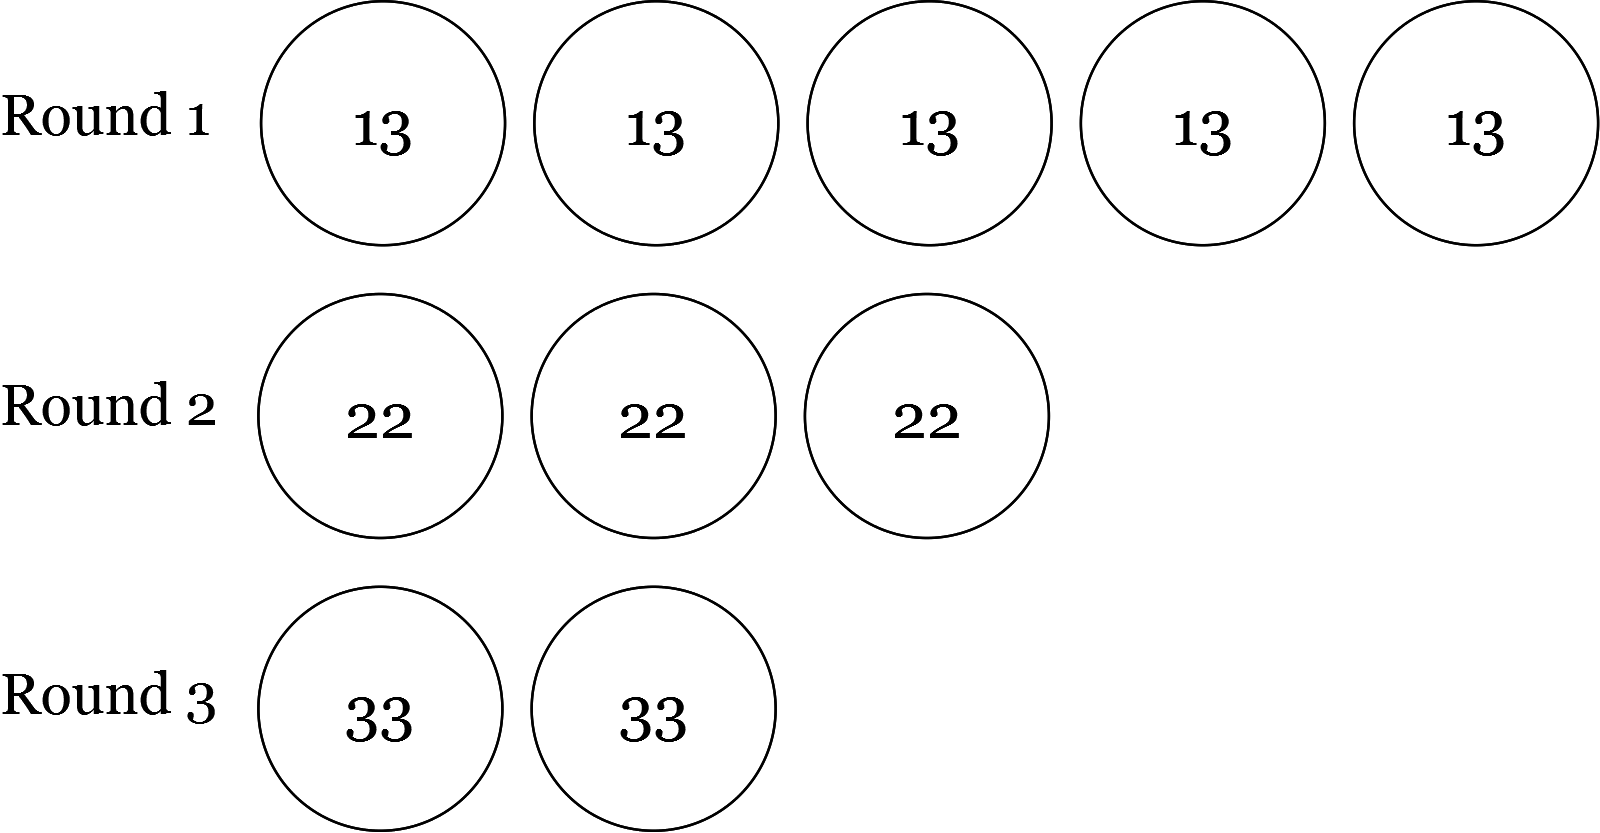
\includegraphics[width=.6\textwidth]{img/seq_halving.png}
	\caption[Sequential Halving example]{Sequential Halving example on 5 arms and a total budget of 200.}
	\label{fig:seq-halving}
\end{figure}

Sequential Halving is a candidate for a recursive definition to be used in MCTS. The algorithm performs well in the cases described in the original article, and samples the best node more frequently than Successive Rejects. Moreover, Sequential Halving currently provides the best bounds on simple regret~\citebay{Karnin13SH}. An MCTS variant that implements Sequential Halving recursively named SHOT~\citebay{Cazenave14SHOT}, is discussed in Chapter~\ref{chap:mctssr}. Unlike Sequential Halving, Successive Rejects has not been used as a selection policy for tree search in current literature, this is open to future research. 

\section{Relation to MCTS}
\label{sec:mabmcts}

\subsection{Upper Confidence Bounds for Trees}
During the MCTS selection step, a policy is required to explore the tree to decide on promising options. For this reason, the widely used Upper Confidence Bound applied to Trees (UCT)~\citebay{kocsis2006bandit} was derived from the UCB1 policy. In UCT, each node is treated as a bandit problem whose arms are the moves that lead to different child nodes. UCT balances the exploitation of rewarding nodes with the exploration of lesser visited ones. Consider a node $p$ with children $I(p)$, then the policy determining which child $i$ to select is defined as:

\begin{equation}
\label{eq:uct}
i^* = \argmax_{i \in I(p)}\left\{ x_i + C \sqrt{ \frac{\ln{n_p}}{n_i}}\right\},
\end{equation}
where $x_i$ is the score of the child $i$ based on the average result of simulations that visited it, $n_p$ and $n_i$ are the visit counts of the current node and its child, respectively. $C$ is an exploration constant to tune. UCT is generally applied when the visit count of a child node is above a threshold~\citebay{coulom2007efficient}. When a node's visit count is below this threshold, a child is selected at random.

Note that UCB1, and consequently UCT, incorporates both exploitation and exploration. After a number of trials, a node that is identified as the empirical best is selected more often. In tree search, this has three consequences:
\begin{enumerate} 
\item Whenever a promising move is found, less time is spent on suboptimal ones. Since UCT is generally time-bounded, it is important to spend as much time as possible exploiting the best moves. Because, by the \emph{MinMax} principle, which states that an agent aims to maximize its minimum gain, on each ply we expect a player to play the best-reply to its parent. 

\item The valuation of any node in the tree is dependent on the values back-propagated. Given that UCT spends less time on suboptimal moves, any values back-propagated are based on increasingly improved simulations, because they are performed deeper in the tree. In fact, given infinite time, UCT converges to almost exclusively selecting nodes with the highest average values.

\item The current value of the node can be falsified by searching deeper. In UCT, each simulation increases the depth of the search, and as such may reveal moves as becoming worse over time due to an unpredicted turn of events. If an expected good move is not reselected often, such ``traps''~\citebay{Ramanujan2010a} are not revealed. More generally, when sampling a game-tree rewards are not necessarily drawn from a fixed distribution.
\end{enumerate}
\newpage
\subsection{Regret in MCTS}

Based on the analysis in the previous subsection, the minimization of cumulative regret is naturally suitable to tree search, and the UCB1 selection policy can be used nearly unaltered in this setting as UCT. However, as is shown in Section \ref{sec:mabprob} there exist two contexts for the multi-armed bandit problem, also to be considered in MCTS. These are:

\begin{enumerate}

\item Each trial results in a direct reward for the agent. As such we want to minimize the number of suboptimal arms pulled in order to achieve a rewards as high as possible. This relates, for example, to slot machines in a casino. Every choice made at each point in the algorithm has a direct effect on the agent's reward. In this case, the reward of the agent is related to the inverse of its \textbf{cumulative regret}.

\item The agent can perform a number of trials, without consequence, in a simulated environment. The agent is allowed $T$ trials in this fashion, after which it must make a recommendation. Based on its recommendation, the agent is rewarded. In this case, the performance of the agent is measured by the \textbf{simple regret} of its recommendation. A low simple regret implies that the recommendation is close to the actual best option.

\end{enumerate}

In most MCTS literature, UCT is used as selection policy~(\cf~\citeay{browne2012survey}), suggesting that the first context applies. However, the second context is a more natural fit when MCTS is used to play games, because the behaviour of the agent in the domain is based solely on its recommendations. Nevertheless, simple regret minimization cannot replace UCT in this case without consideration. Unlike in an MAB, sampling does have an immediate impact on performance in MCTS because reward distributions can be non-stationary. 
Spending more time on suboptimal moves when descending the tree decreases the amount of time available to explore nodes expected to have high utility. Moreover, since all values are back-propagated, we risk under-evaluating ancestors based on sampling nodes that are known to be bad. This trade-off was also shown in~\citebay{tolpin2012mcts}, where the authors use a measure based on the Value of Information (VOI) to determine whether to exploit an expected good move, or continue exploring others. This trade-off is also described as a ``separation of exploratory concerns'' in Best Recommendation with Uniform Exploration (BRUE)~\citebay{Feldman12BRUE}.

The general performance of MCTS may be improved by applying a strategy that is focused on minimizing simple regret fast near the root, rather than cumulative regret. Because the recommendation made by MCTS is based on the values of the root's children, assuming that simple regret is a better measure of the quality of a given decision at time $T$, and that we can apply both the aforementioned contexts to search in a specific manner, the algorithms discussed in this chapter may improve the performance of MCTS when they are combined with UCT. In this manner, the benefits of lower bounds on simple regret for the recommendation at the root will originate from results back-propagated from selections made by UCT deeper in the tree, using both methods in their appropriate context.

In the next chapter, MCTS variants designed to (partially) minimize simple regret are discussed. Subsequently, in Chapter~\ref{chap:hybmcts}, a new search technique is proposed that uses both simple and cumulative regret minimizing policies at appropriate segments of the MCTS tree. Using this technique, we can determine whether whether the assumption holds that preferring simple over cumulative regret minimization near the root is both practical, and improves overall performance.

% -----------------------------------------------------------------------------
% ------------------- ::::::: Simple Regret In MCTS ::::::: -------------------
% -----------------------------------------------------------------------------
\chapter{Simple Regret in MCTS}
\label{chap:mctssr}

\begin{chaptercontents} A discussion on MCTS variants using simple regret minimizing selection policies. This chapter serves as introduction and inspiration to the next in which the new search technique, which combines different selection policies, is detailed.
\end{chaptercontents}

\section{Introduction}
Since the introduction of MCTS~\citebay{kocsis2006bandit} and its subsequent adoption by games researchers~(\cf~\citeay{browne2012survey}) UCT, or some variant thereof, has become the ``default'' selection policy. Since the introduction of simple regret~\citebay{Bubeck11Pure}, more MCTS research has been performed using simple regret as the minimizing metric.

\citeaby{Feldman12BRUE} have proposed an algorithm named BRUE, developed to guarantee an exponential rate of reduction of simple regret. Rather than building a connected tree such as MCTS, BRUE generates non-connected nodes based on a switching function. The authors mention that the algorithm is a possible replacement for UCT. In \citeaby{Feldman13}, BRUE is extended such that it may be used in more practical domains. Importantly, the proposed BRUE\textsubscript{$\mathcal I$} can be used without specifying a fixed horizon, rather it builds a tree connected to the root incrementally. Therefore, based on experimentation with BRUE and BRUE\textsubscript{$\mathcal I$} in the games discussed in this thesis, no improvement was shown over UCT. Based on these findings, the algorithm is not discussed in this chapter.

Rather than optimizing either simple or cumulative regret throughout the MCTS tree,~\citeaby{tolpin2012mcts} propose a technique in which simple regret is minimized using either a modified version of UCB or a $\frac{1}{2}$-greedy policy only at the root, and UCT throughout the rest of the tree. Similar to BRUE, the authors developed this algorithm for solving \emph{Markov decision processes}. SHOT~\citebay{Cazenave14SHOT} is an MCTS algorithm based on Sequential Halving~\citebay{Karnin13SH}. This algorithm was developed to provide a speed-improvement over UCT, allowing more simulations per second to be performed and thereby increasing performance in game-play. SHOT spends less time in the tree back-propagating values from leaf to root because it assigns a potentially large budget of play-outs to each node. This means that accumulated values are back-propagated in the tree, instead of a single win or loss after each play-out.

\vspace{2 mm}
Two MCTS variants are discussed in this chapter, as their approaches lead to key insights for the development of a hybrid MCTS. First, in Section \ref{sec:srmcts}, the so-called Simple Regret + Cumulative Regret (SR+CR) scheme proposed by~\citebay{tolpin2012mcts} is discussed. Next, in Section \ref{sec:SHOT}, the recently introduced SHOT~\citebay{Cazenave14SHOT} is detailed. Both algorithms form the foundation of Hybrid MCTS (H-MCTS), which is introduced in the next chapter.
\newpage
\section{MCTS Based on Simple Regret}
\label{sec:srmcts}

\citeaby{tolpin2012mcts} give the same arguments presented in Chapter \ref{chap:mab}: that when MCTS is used in a the context of search in an MDP, \emph{`` it is usually only the final 'arm pull' (the actual move selection) that collects a reward, rather than all 'arm pulls' ''}~\citebay{tolpin2012mcts}. Moreover, the exploitation of high valued nodes is not preferable in all circumstances. Rather, more time should be spent exploring the alternatives. The hypothesis of the article is that since only the children of the root represent an action to be taken in the domain, a selection policy that minimizes simple regret at the root, and UCT throughout the rest of the tree, should have better performance than using only UCT.

Two selection policies with lower bounds than UCT on simple regret were constructed by the authors for the purpose of selecting nodes at the root.
\begin{enumerate}
\item $\frac{1}{2}$-greedy, a policy that selects a move at random half of the time, and the current empirical best the other half. This policy offers an exponentially decreasing simple regret.
\item ${UCB}_{\sqrt{.}}$, which is similar to UCT, however the logarithm in the numerator in the upper confidence bound is replaced by a square root.
\begin{equation}
\label{eq:uctsqrt}
i^* = argmax_{i \in I(p)}\left\{ v_i + C \sqrt{ \frac{\sqrt{n_p}}{n_i}}\right\}
\end{equation}
This selection policy has a super-polynomially decreasing simple regret~\citebay{tolpin2012mcts}.
\end{enumerate}
In both cases, the recommendation made by the algorithm is based on the node with the highest value at time $T$.

Next, a two-stage sampling scheme named SR+CR uses one of the above policies at the root, and UCT in the rest of the tree. In Algorithm \ref{alg:tsmcts}, the scheme proposed by the authors is given in the context of game-play. Although originally, the algorithm was designed for maximizing rewards on each ply, it is presented in th negamax context such that it applies to games.
\IncMargin{1em}
\RestyleAlgo{boxruled}
\begin{algorithm2e}[b]
\setstretch{1.2}
	\KwIn{node $p$, current search depth}													
	\func{srcr-mcts}(node $p$, $depth = 1$):														\;
	\Indp							
	\lIf{isLeaf($p$)}{Expand($p$)}
	\eIf{$depth = 1$} {
	select child $i$ using $\frac{1}{2}$-greedy or ${UCB}_{\sqrt{.}}$								\;
	}
	{
	select child $i$ using UCT 																		\;
	}

    \eIf{isLeaf(i)} {
    	$r \gets$ {\sc playout}$(i)$ 																\;
    	\func{update} node $i$ with $r$																\;
    }
    {
    	$r \gets$ -\func{srcr-mcts}($i$, $depth + 1$)												\;
    }	
    \func{update} node $p$ with $r$																	\;
	\Indm
    \KwRet{$r$}
  \caption[Two-stage Monte-Carlo Tree Search]{Two-stage Monte-Carlo Tree Search~\protect\citebay{tolpin2012mcts}. \label{alg:tsmcts}}
\end{algorithm2e}
\DecMargin{1em}

The selection policies were empirically validated to have lower simple regret than UCB in MABs. Moreover, the SR+CR scheme was shown to have lower simple regret in the MDP sailing domain. Particularly, the scheme was more advantageous when the number of nodes at the root are higher. Although the SR+CR scheme and two-stage MCTS were not developed for game-play, it holds merit to attempt to replicate the favourable results presented in games. Since, as the authors argue, only the options given at the root collect any true reward from the domain, and this is the case in both MDP domains and games. The algorithm presented was implemented for Amazons, Breakthrough, NoGo and Pentalath. However, using either of the two selection methods proposed declined performance when competing against UCT in preliminary experiments.

\section{Sequential Halving Applied to Trees}
\label{sec:SHOT}

A recent addition to simple regret techniques in MCTS is Sequential Halving applied to Trees (SHOT) \citebay{Cazenave14SHOT}. The algorithm is presented as a ``faster'' version of MCTS. Instead of using UCT and backing up values after each simulation from leaf to root, SHOT uses Sequential Halving throughout the tree. This essentially turns MCTS into an iterative deepening, depth first search. The main benefit the author points out is that SHOT spends much less time in the tree, updating and back-propagating values. Consequently, an optimized engine with fast play-outs can perform more simulated games per turn using SHOT than it could with UCT. In practice it means that for the same number of play-outs SHOT is approximately twice as fast as UCT. SHOT allocates a
possibly large number of play-outs to the possible moves. This makes it quite easy to parallelize without loss of information and without changing the behaviour of the algorithm.

In the MAB context, Sequential Halving is run once, but in MCTS, nodes can be revisited, and therefore Sequential Halving is ``restarted'' upon revisiting a node. Define a \emph{cycle} as one full iteration of Sequential Halving which starts on line~\ref{shot:cycle}, and a \emph{round} as a sub-iteration over a given subset of $S$ which starts on line~\ref{shot:round}, in Algorithm~\ref{alg:shot}. Because any number of cycles may be started on a given node, care must be taken that budget is divided such that after any cycle the visit counts of all nodes are as if only one cycle was run. Therefore, when dividing the budget on line \ref{shot:budgeting} the current budget spent is added to the allocated budget, essentially overestimating the total budget available. Next, on line \ref{shot:topoff} only the budget that exceeds the current child's visits is allocated. This is illustrated in Figure \ref{fig:shot-topoffs}, where a node that was previously visited 64 times starts a new cycle with a budget of 128. The new budget per arm is: $\floor[\big]{\frac{64 + 128}{4\times\ceil{log_2{4}}}} = 24$. However, since the second and fourth child have previously been assigned a total budget of 24, only the first and third node are assigned $24-8=16$ budget.

\begin{figure}[h]
	\centering
	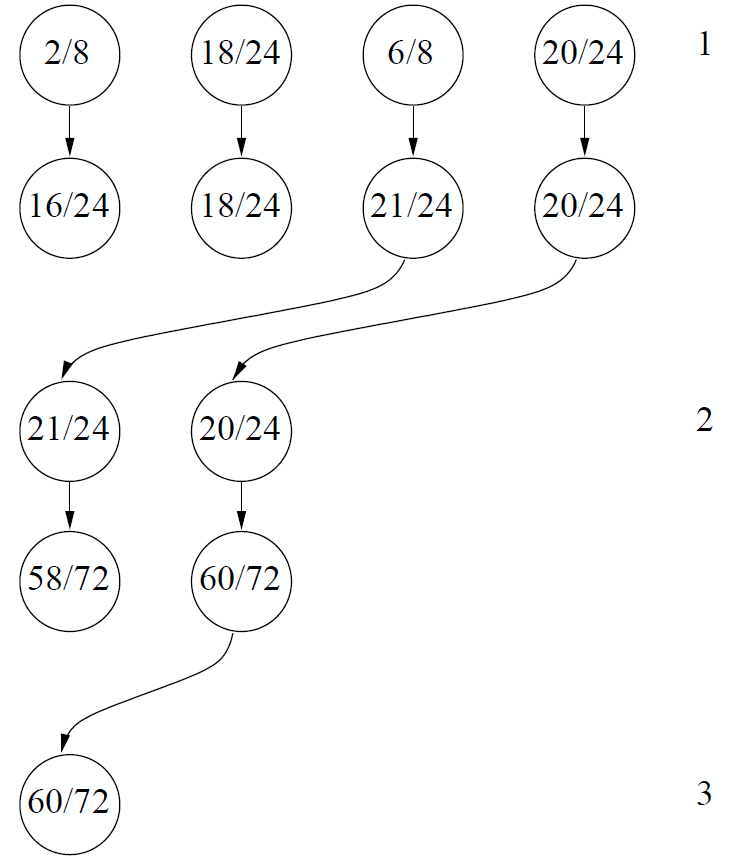
\includegraphics[width=.3\textwidth]{img/shot_topoffs.png}
	\caption[SHOT budget division example]{Division of 128 play-outs. The current node was previously visited 64 times \\ \protect\citebay{Cazenave14SHOT}.}
	\label{fig:shot-topoffs}
\end{figure}

SHOT was demonstrated to outperform UCT in NoGo, both on $9\times9$, and $19\times19$ boards, with win-rates between $75\%$ and $100\%$~\citebay{Cazenave14SHOT}. However, based on the results in the article and Chapter \ref{chap:experiments}, these results were due to SHOT being significantly faster than UCT, when both algorithms are given the same budget of play-outs, different results are achieved.

Although in the original article SHOT is presented with the use of a transposition table instead of a tree, in Algorithm \ref{alg:shot} a version of SHOT using a tree of game states is presented.

\newpage
\IncMargin{1em}
\RestyleAlgo{boxruled}
\begin{algorithm2e}[ht]
\setstretch{1.1}
	\KwIn{node $p$, allocated budget $budget$}
	\KwOut{tuple containing the number of visits, $p1$ and $p2$ wins, budget used}
	\func{shot}(node $p$, $budget$):													\;
	\Indp
	\lIf{isLeaf($p$)}{$S\gets$ \func{expand}($p$)}					
	$t_p \gets \tuple{0,0,0,0}$															\;
	\If{isTerminal($p$)}{																	\label{shot:terminal}
		\func{update} $t_p$, with $budget$ wins for the appropriate player and $budget$ visits 					\;
		\KwRet{$t_p$}																	\;
	}
	\If{budget = 1} {																		\label{shot:playout}
		$r \gets$ \func{playout}($p$)													\;
		\func{update} $t_p$, with 1 budget used, 1 win for the appropriate player, and 1 visits					\;
		\KwRet{$t_p$}																	\;
	}
	\If{$|S|$ = 1} {
		$n_0 \gets$ the single element in $S$											\;
		$t_p \gets $ \func{shot}($n_0$, $budget$)											\;
		\func{update} $p$ with $t_p$													\;
		\KwRet{$t_p$}																	\;	
	}
	$s \gets |S|$, $S_0 \gets S$, $b_u, b, k \gets 0$									\;
	\While{$s >$ 1 \textbf{and} $b_u < budget$} {											\label{shot:cycle}
	$b \gets b + \displaystyle\max{\left(1, \floor[\bigg]{\frac{p.budgetSpent + budget}{s\times\ceil{log_2{|S|}}}}\right)}$ \;	\label{shot:budgeting}
		\For{i=1 \emph{\KwTo} s}{															\label{shot:round}
			$n_i \gets$ node $n$ at rank $i$ of $S_k$									\;
			$b_i \gets b - n_i.visits$													\;  \label{shot:topoff}
			\If{$b_i > 0$} {
				\If{$p$ is root \textbf{and} $i = 0$ \textbf{and} $s = 2$} {
					\tcp{Spend any left-over budget on the empirically best node}
					$b_i \gets \max{(b_i, budget - b_u - (b - n_1.visits))}$				\;
				}
				$b_i \gets \min{(b_i, budget - b_u)}$										\;
				$\tuple{v, w_1, w_2, b_{u, n_i}}_i \gets$ \func{shot}($n_i$, $b_i$)			\;
				\func{update} $p, b_u,$ and $t_p$ with $\tuple{v, w_1, w_2, b_{u, n_i}}_i$	\; \label{shot:tp_update}
			}
			break if $b_u \geq budget$													\;
		}
		$k \gets k + 1$																		\;
		$S_{k} \gets$ $S_{k-1}$ sorted in descending order									\;
		$s \gets \ceil{\nicefrac{s}{2}}$													\;
	}
	\func{update} $p.budgetSpent$ with $b_u$												\; \label{shot:budg_spent}
	\Indm
	\KwRet{$t_p$}
  \caption[Sequential Halving applied to Trees (SHOT)]{Sequential Halving applied to Trees (SHOT)~\protect\citebay{Cazenave14SHOT}. \label{alg:shot}}
\end{algorithm2e}
\DecMargin{1em}

\newpage
SHOT recursively performs Sequential Halving until either a terminal state is encountered (line \ref{shot:terminal}), or the available budget for the current node is 1 (line \ref{shot:playout}). Because multiple play-outs can be performed from a single recursive call, a tuple $t_p$ is maintained containing: 1) the budget used $b_u$, 2) the number of wins per player $w_1$ and $w_2$, and 3) the number of visits $v$. $v$ differs from $b_u$, because visiting a terminal node spends no budget, but performing a play-out does, and in both cases the visit count of the node should be increased. On line~\ref{shot:tp_update}, $p$ is updated with the results returned from the recursion, $b_u$ is updated with the total budget used by play-outs, and $t_p$ is updated with all returned values. On line~\ref{shot:budg_spent} the total budget spent at the current node is incremented. This value is used to determine the budget of the next round of SHOT.

A disadvantage of SHOT is that it cannot be terminated any time, and requires a-priori knowledge of the available budget. The pure exploration policies discussed in Chapter \ref{chap:mab} guarantee a low simple regret on the recommendation only after all available $T$ simulations are performed. Therefore, they cannot be terminated, or asked for a reasonable recommendation before this limit is reached.

This leads to another concern when using any pure exploration policy recursively. As discussed in Chapter \ref{chap:mab}, UCT has the advantage of almost exclusively selecting the best node over time, giving the formal guarantee that suboptimal nodes are selected at most $O(\ln{n})$ times. This ensures that over time, values accumulated at nodes approximate the value of the best-reply to the node's move. With a policy such as Sequential Halving this guarantee is related to the available budget and the branching factor. In fact, the two empirically best nodes are sampled equally, however different their reward may be. Moreover, for a node with a set of children $S$, the worst $\frac{|S|}{2}$ of these are sampled at least at total of $\floor{\frac{T}{\ceil{log_2{|S|}}}}$ times. In many games there are only a handful of good moves given a position, and to evaluate a node the value of its move's best-reply must be found. By using Sequential Halving throughout the tree, values back-propagated do not converge in the same manner as UCT, as such, values of internal nodes are constituted of more overall averages over their children.

% --------------------------------------------------------------
% ------------------- ::::::: H-MCTS ::::::: -------------------
% --------------------------------------------------------------
\chapter{A Hybrid MCTS}
\label{chap:hybmcts}
\begin{chaptercontents}
The main contribution of this thesis, a hybrid version of MCTS named H-MCTS, which combines simple and cumulative regret minimizing selection policies into a single search technique.
\end{chaptercontents}
\section{Introduction}
As a selection policy for MCTS, UCT minimizes cumulative regret over time throughout the tree. At internal nodes, minimizing cumulative regret ensures a node with a high expected reward is visited more often. UCT converges asymptotically to a greedy selection policy, where at each iteration only the expected best node is selected. In effect, the average rewards at parent nodes converge to the maximum over their children, \ie UCT converges to maximum back-propagation on a stable distribution~\citebay{kocsis2006bandit}. Secondly, UCT ensures that search time is divided efficiently, limiting the number of  suboptimal nodes selected by $O(\ln(n))$ where $n$ is the number of trials~\citebay{auer2002using,kocsis2006bandit}. However, such a selection policy offers a simple regret that decreases at best polynomially fast~\citebay{Bubeck11Pure}. These two properties are not only practical when long deliberation times are feasible, rather, it is possible to terminate UCT at any time to obtain a reasonable approximation of the utility of a decision. During search this means that at each ply and at any time, MCTS can be asked for a best response to a parent's move.

In contrast, pure exploration algorithms, designed to minimize simple regret in multi-armed bandits such as Successive Rejects~\citebay{audibert2010best} and Sequential Halving~\citebay{Karnin13SH}, discussed in Chapter~\ref{chap:mab}, explore all options without specifically exploiting the best one. This results in a lower bound on simple regret only after all simulations have been performed. As such, to be used effectively, these algorithms can not be terminated at \emph{any time}, and have a lower formal guarantee on the number of suboptimal selections made. Moreover,~\citeaby{Bubeck11Pure} have shown that at moderate deliberation times, a modified UCB selection policy, which includes an exploration constant not unlike UCT, resulted in a better bound on simple regret than algorithms designed to minimize it. Relating these findings to MCTS, and assuming that given sufficient time, minimizing simple regret gives a lower simple regret than UCT, we may choose to use a simple regret minimizing algorithm whenever sufficient trials can be performed, and switch to UCT when the computational budget is smaller.

Inspired by the analysis and discussions in Chapters \ref{chap:mab} and \ref{chap:mctssr}, a new MCTS variant is proposed named Hybrid MCTS (H-MCTS). H-MCTS initializes with an exploratory depth-limited search, applying a specific simple regret minimizing policy. After reaching a node where computational budget per node is smaller than a set limit, the algorithm switches to the UCT selection policy. 
\vspace{2 mm}

Section \ref{sec:hybmcts} gives an introduction and analysis of H-MCTS. Next, Section \ref{sec:hybmctssolver} details the implementation of MCTS-Solver~\citebay{Winands2008}, designed to solve positions within the tree, for H-MCTS. Finally, in Section \ref{sec:ulb_h-mcts}, an enhancement for SHOT and H-MCTS is introduced that reduces the number of unpromising nodes selected based on whether their upper confidence bounds overlap with their current empirically best sibling's lower confidence bound.
\newpage
\section{Hybrid MCTS}
\label{sec:hybmcts}

Recall that in the MAB context, in which simple regret minimization is appropriate, only the final recommendation made by an algorithm has an effect on the agent's reward. In game play this holds for the nodes of the search tree at the first ply. Only after performing all simulations is a recommendation made which affects the state of the game being played. Nodes deeper in the tree have an implicit effect on this decision. Because the shape of an MCTS tree is directly related to the potential reward of internal nodes, promising nodes are selected more often to grow the tree in their direction. This both reinforces the confidence of the reward of promising nodes, but also ensures that their reward can be falsified based on results deeper in the tree.

\begin{figure}[ht]
	\centering
	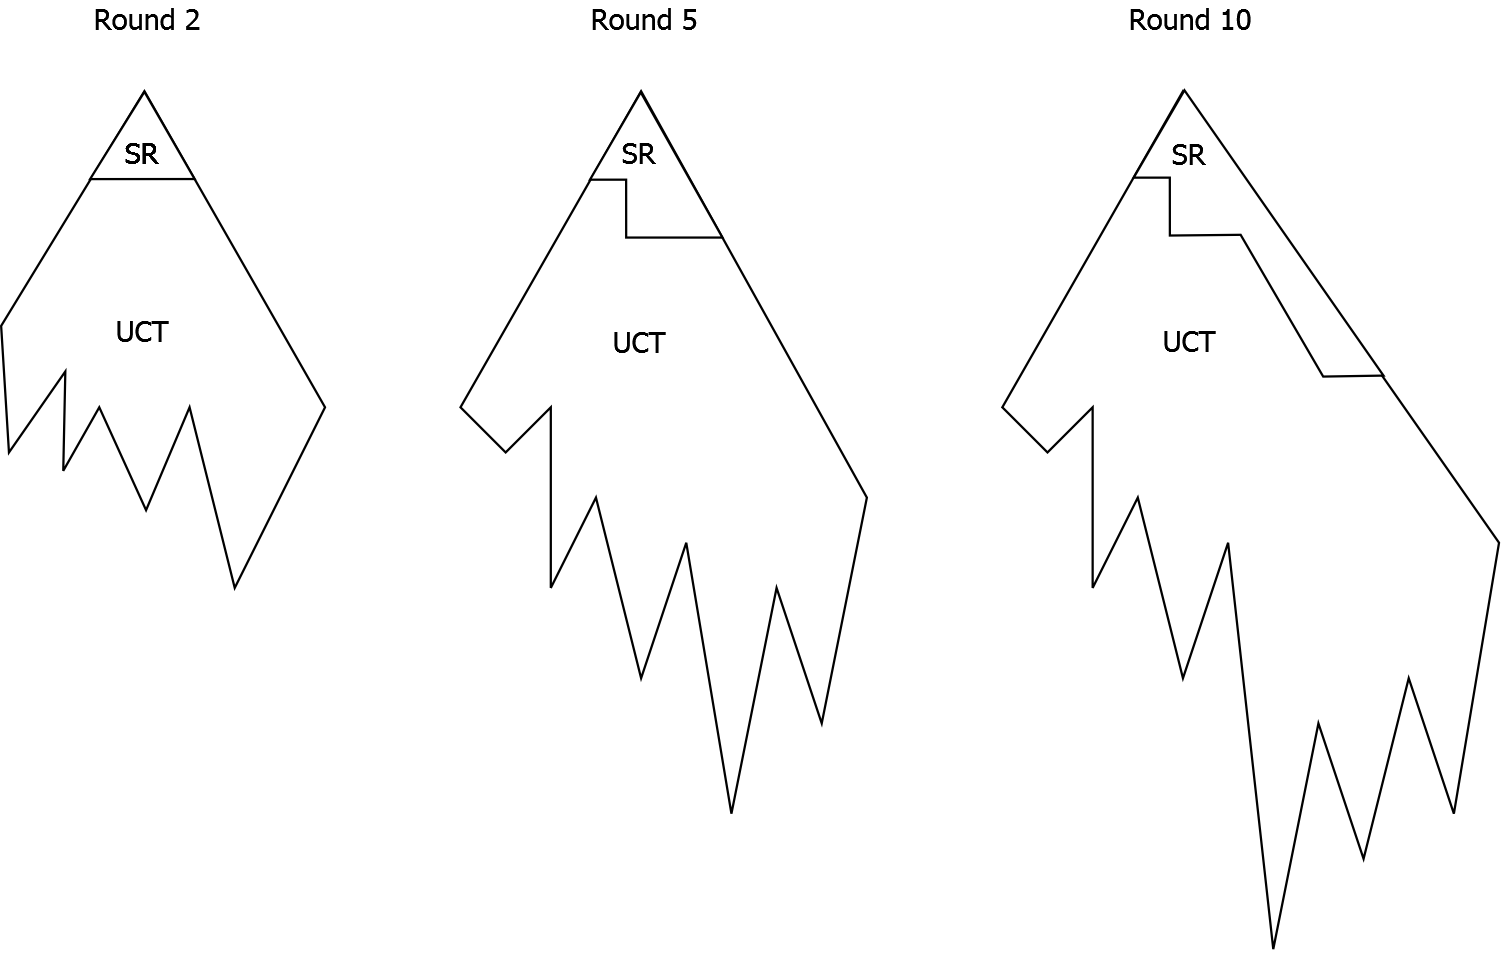
\includegraphics[width=.75\textwidth]{img/H-MCTS.png}
	\caption[Hybrid MCTS tree progression]{Example progression of H-MCTS. In the top part of the tree (SR), simple regret is minimized, in the lower part UCT minimizes cumulative regret. The rounds represent the Sequential Halving round at the root.}
	\label{fig:h-mcts_trees}
\end{figure}

Treating a game tree as a recursive multi-armed bandit thus reveals different objectives for the distinct plies of the tree. At the root, simple regret should be as low as possible, since the recommendation of the algorithm is based on the first ply of the tree. Further down, we want to both sample efficiently, avoiding time wasted on bad options, and back-propagate correct values from leafs to their ancestors. Where the former can be achieved by using selection policies such as Successive Rejects or Sequential Halving, the latter, as discussed in Section \ref{sec:mabmcts} is inherently performed by UCT. Intuitively, this leads to the belief that we should only minimize simple regret at the root, and use UCT throughout the rest of the tree, as suggested by~\citeaby{tolpin2012mcts}. 
However, considering that at any node, based on the MinMax principle, we want to find the \emph{best reply} to the action of the parent. It may also be beneficial to ensure a low simple regret on that particular move because this could intrinsically lead to an improved evaluation of the parent. Using the SHOT technique, we can apply Sequential Halving recursively, essentially combining recursive simple and cumulative minimization in a single search tree, as depicted in Figure~\ref{fig:h-mcts_trees}.

\begin{figure}[ht]
	\centering
	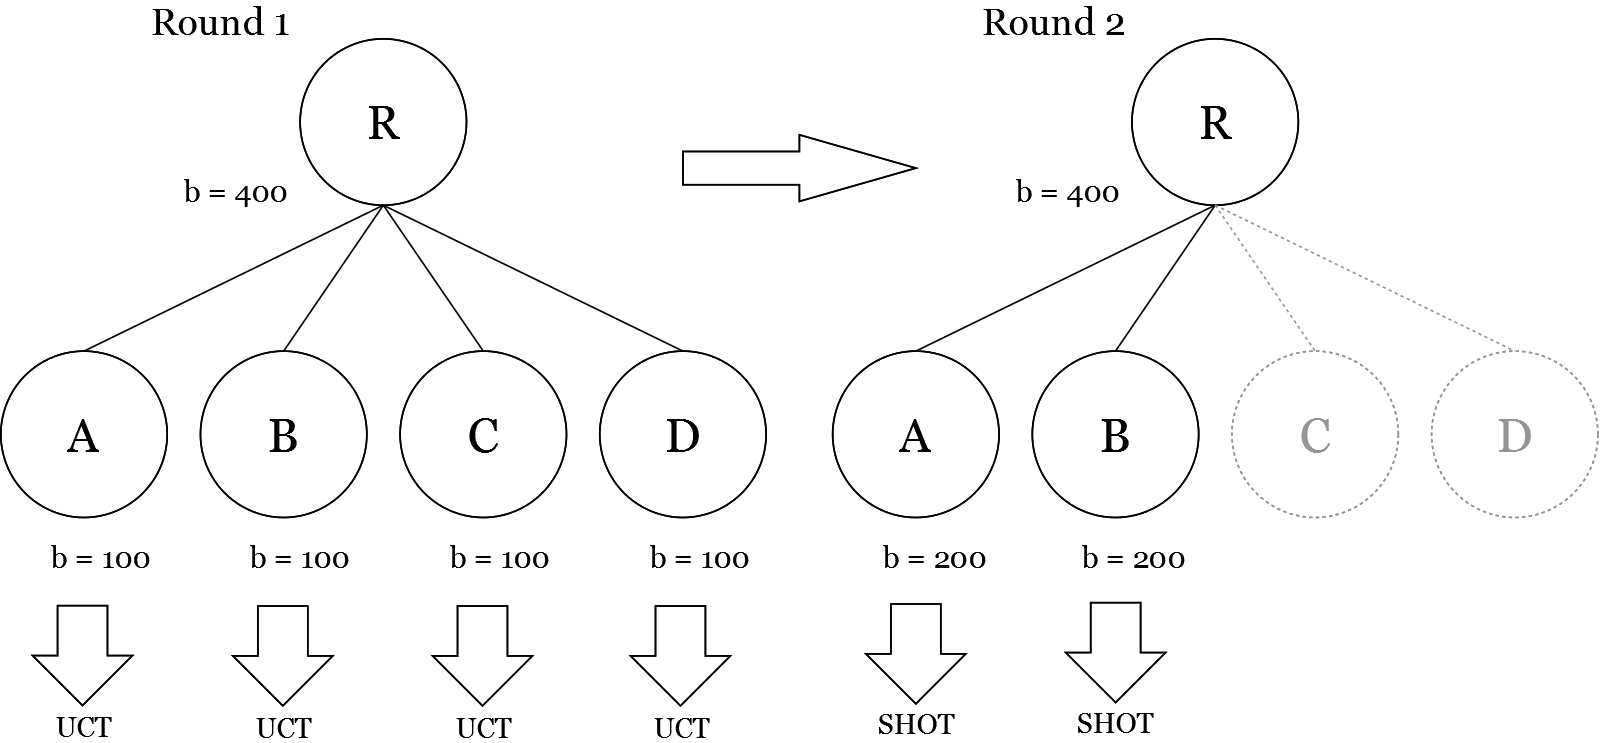
\includegraphics[width=.75\textwidth]{img/H-MCTS_Rounds.png}
	\caption[Hybrid MCTS example rounds]{Example rounds of H-MCTS with a budget limit $B = 150$. During the first round SHOT is used only at the root R. In round 2, the budget per node is higher, and SHOT is used recursively at nodes A and B.}
	\label{fig:h-mcts_rounds}
\end{figure}

Using a selection policy based on both SHOT and UCT, H-MCTS combines simple and cumulative regret minimization in a tunable algorithm. \citeaby{Bubeck11Pure} have shown that given a low sampling budget, UCB empirically realizes lower simple regret. Therefore, the proposed technique switches from Sequential Halving to UCT whenever the computational budget is below the budget limit $B$. Consequently, the search tree is composed of a \emph{simple regret tree} at the root, and \emph{UCT trees} rooted at the leafs of the simple regret tree. As shown in Figure~\ref{fig:h-mcts_trees}, initially the simple regret tree is shallow because the computational budget per node is small. Later, when the budget per node increases due to nodes being removed from selection as per Sequential Halving, the simple regret tree grows deeper. Note that because the root's children are sorted in descending order, the left part of the simple regret and UCT trees are always the deepest, since those UCT trees are selected the most, see Figure~\ref{fig:h-mcts_rounds}.
\newpage
\IncMargin{1em}
\begin{algorithm2e}
\setstretch{1.1}
	\KwIn{node $p$, allocated budget $budget$}
	\KwOut{$t_p$: number of play-outs, $p1$ and $p2$ wins}
	\vspace{0.1cm}
	\func{h-mcts}(node $p$, $budget$):												\;
	\Indp
	\lIf{isLeaf($p$)}{$S\gets$ \func{expand}($p$)}					
	$t_p \gets \tuple{0,0,0}$														\;		
	\If{isTerminal($p$)}{															\label{h-mcts:terminal}
		\func{update} $t_p$, with $budget$ wins for the appropriate player, and $budget$ visits							\;
		 \KwRet{$t_p$}
	}
	$b \gets \max{\left(1, \floor[\bigg]{\frac{p.budgetSpent + budget}{s\times\ceil{log_2{|S|}}}}\right)}$ \; \label{h-mcts:budgetlimit}
	\If{not isRoot($p$) \textbf{and} $b < B $}{
		\For{i=0 \emph{\KwTo} budget}{
			$\tuple{v, w_1, w_2}_i \gets$ \func{uct}($p$)							\;
			\func{update} $p, t_p$ with $\tuple{v, w_1,w_2}_i$						\;
		}
		\KwRet{$t_p$}
	}
	$b_u, k \gets 0$\; $S_0 \gets S$\; $s \gets |S|$								\;
	\Repeat{$b_u \geq budget$ \textbf{or} $s < 2$} {								\label{h-mcts:shot}
		\For{i=1 \emph{\KwTo} s}{
			$n_i \gets$ node $n$ at rank $i$ of $S_k$								\;			
			\If{$b > n_i.visits$} {
				$b_i \gets b - n_i.visits$											\;
				\lIf{$i = 0$ \textbf{and} $s = 2$} { $b_i \gets \max{(b_i, budget - b_u - (b - n_1.visits))}$ }
				$b_i \gets \min{(b_i, budget - b_u)}$								\;
				$\tuple{v, w_1, w_2}_i \gets$ \func{h-mcts}($n_i$, $b_i$)			\;
				\func{update} $p, b_u$, and $t_p$ with $\tuple{v, w_1, w_2}_i$		\;	\label{h-mcts:update}
			}
			break if $b_u \geq budget$												\;
		}
		$k \gets k + 1$																\;
		$S_{k} \gets$ $S_{k-1}$, with the first $s$ elements sorted in descending order	\;	\label{h-mcts:sort}
		$s \gets \ceil{\nicefrac{s}{2}}$										\;
		$b \gets b + \max{\left(1, \floor[\bigg]{\frac{p.budgetSpent + budget}{s\times\ceil{log_2{|S|}}}}\right)}$\;
	}
	\func{update} $p.budgetSpent$ with $b_u$										\;
	\Indm
	\KwRet{$t_p$}
  \caption{Hybrid Monte-Carlo Tree Search (H-MCTS). \label{alg:h-mcts}}
\end{algorithm2e}
\DecMargin{1em}

H-MCTS is outlined in Algorithm~\ref{alg:h-mcts}. Similar to UCT and SHOT, on line~\ref{h-mcts:terminal} terminal conditions are handled, followed by the main feature of the algorithm on line~\ref{h-mcts:budgetlimit} where the initial simulation budget $b$ for each child of the current node is computed. Based on $b$, a decision is made whether to progress into the UCT tree if $b<B$ or, if $b \geq B$ to continue with SHOT. Note that the $b<B$ check is overridden at the root, since only one cycle is initiated there. Assuming the allocated budget is large, at the root simple regret minimization is preferred over cumulative regret minimization. From line~\ref{h-mcts:shot} the algorithm is similar to the Sequential Halving portion of SHOT. As in SHOT, because multiple play-outs are back-propagated in a single descent from root to leaf, the algorithm returns a tuple $t_p$, which contains: 1) the number of visits $v$, and 2) the number of wins per player $w_1$ and $w_2$. On line~\ref{h-mcts:update}, the budget used $b_u$ is incremented by $v$ from the results returned by the recursion. Moreover, the current node's statistics are updated, alongside the cumulative tuple $t_p$, which are returned to the node's parent. UCT also maintains a tuple of statistics such that it can return the same $t_p$ to the simple regret tree. For the UCT tree, any implementation can be used, as long as it is adapted to return $t_p$ and update the $budgetSpent$ value alongside the usual node's visit count because any UCT node in the tree can be ``converted'' to a simple regret node at any time, when $b>B$ on line~\ref{h-mcts:budgetlimit}. 

As with MCTS, H-MCTS can be separated in four discrete steps:
\begin{enumerate}
\item \textbf{Budgeting}: A budget is determined for each child. Based on the budget, we enter the UCT tree, or remain in the simple regret tree. If we enter the UCT tree, the four basic MCTS steps apply.
\item \textbf{Selection}: In the simple regret tree, nodes are sampled based on Sequential Halving. Nodes in the simple regret tree are assigned a budget, to be spent in their rooted UCT tree, in which play-outs are initiated.
\item \textbf{Removal}: Based on the results obtained, children are removed from selection. A new Sequential Halving round starts with half of the best children from the previous round. If the budget is spent, the currently accumulated results are back-propagated.
\item \textbf{Back-propagation}: Since H-MCTS is performed depth-first, the final result is only available after all budget is spent. This results in simultaneous back-propagation of numerous results in the simple regret tree.
\end{enumerate}

H-MCTS shares its disadvantage of not being able to return a recommendation at any time with SHOT. It must know its exact computational budget beforehand. However, it does make use of the fact that UCT is any-time. Suppose a node were selected and expanded by H-MCTS. Then, at each time in the simple regret tree, nodes have an appropriate value based on the results back-propagated by UCT. Thus, when SHOT finishes a round by sorting the nodes by their accumulated values on line~\ref{h-mcts:sort}, UCT's any-time property ensures nodes have a representative value.

When all $T$ simulations have been performed, H-MCTS recommends the single remaining node $n_0 \in S$ at the root. Note that this is not necessarily the one with the highest value, it is possible that the best node's value has decreased after several rounds. However, we cannot assume that the values of the previously removed nodes do not also decrease given more samples. Therefore, because most samples were spent on $n_0$, we are the most confident in its value. Other nodes with less visits may have higher values, but the confidence in these values is much lower. A possible solution to this problem presents itself in the manner that $S_k$ is constructed, on line~\ref{h-mcts:sort}. An alternative would be to setup each round's subset of nodes as follows: $S_k \gets S$ sorted in descending order. This way, nodes that were previously removed from selection can `return', and replace nodes whose value decreased.

To a lesser extent, H-MCTS also shares the speed benefit of SHOT. However, because a large part of the search tree is composed of the UCT tree, based on the budget limit $B$ H-MCTS still spends more time in the tree than SHOT overall. However, given a lower budget limit $B$, H-MCTS can be made to run faster by increasing the ratio of the simple regret tree related to the UCT tree.

\subsection{Budgeting}
In the scheme presented, a limit on the available budget determines whether to continue in the simple regret tree. However, other methods, such as a fixed depth limit for the simple regret tree, or a time-partitioned method can be viable. However, based on the simple regret theory in MABs, pure exploration methods only provide empirically better simple regret than UCB, given a sufficiently large budget. Given a small budget, UCB with a properly tuned constant should be preferred~\citebay{Bubeck11Pure}. Directly applying this result to MCTS means that whenever the available budget is low, UCT with a properly tuned constant should be preferred to reduce simple regret.

The budget limit $B$ is compared to SHOT's budget allocation:
\begin{equation}
	b = \floor[\bigg]{\frac{p.budgetSpent + budget}{s\times\ceil{log_2{|S|}}}},
\end{equation}
which includes the budget previously spent at the node.

Whenever a Sequential Halving round can be initiated with a budget per child higher than $B$, we continue in the simple regret tree. Otherwise the budget is assigned to UCT, which runs $b$ simulations, and returns the result of their play-outs. Play-outs are only ever initiated in the UCT tree, because UCT immediately takes advantage of the values stored at nodes, whereas Sequential Halving selects all children $b$ times in the first round regardless of their prospects. 

\subsection{Selection}
Selection is performed by uniformly distributing the assigned budget according to the method used in SHOT. However, in H-MCTS any left-over budget is spent in the final round of Sequential Halving, as opposed to spending all residual budget at the root's best child. This ensures that internal nodes' best-replies are selected more often, improving the confidence in their valuation, and of their parent's values.

Note that although Sequential Halving is presented as the simple regret algorithm in H-MCTS, it is certainly possible to replace it with a different selection policy, such as Successive Rejects, or another form of sequential reduction of nodes.

\subsection{Removal}
Since it is possible to visit a node more than once with a new budget, children are merely ``excluded'', instead of removed, from selection. The current list of selection candidates $S_k$ consists of all children sorted from 0 to $s$. Whenever a new budget is assigned to a node, all the previously excluded children are returned so $S_0$, and a new Sequential Halving cycle can begin.

\subsection{Back-propagation}

Typically in MCTS, results of all play-outs are back-propagated and accumulated at every ancestor of the expanded leaf, \ie \emph{average back-propagation}. To determine a node's value, its descendants should be selected such that the (expected) best ones are sampled most often. In the classic MiniMax case, a node's value is determined by the value of its best-reply. In MCTS, this idea is not explicit: over time a node's value converges to the value of its best-reply. However, when a node is insufficiently sampled, the general approach assigns it the current average value of its children.

Whereas UCT selects only promising nodes when it can, Sequential Halving samples all nodes in the current subset, each round. This means that the statistics collected at the parent of a given node do not reflect the best-reply to its move. Moreover, unlike Sequential Halving, UCT can be asked for a recommendation at any time, this means that a node explored by UCT has a representative value at any time. With Sequential Halving, intermediate averages of a node explored by the selection policy may be under-evaluated. Recall that the best and second best children are sampled equally often, in case there exists only a single best-reply to a parent's move, this means that its value never reflects that of its best-reply. This is depicted in an example in Figure~\ref{fig:seq_halv_bp}, where the parent is under-evaluated as it is an expected win for the player to move, whereas the parent's value represents a predicted loss. When this node is reselected with new budget to allocate, this situation does not improve, because Sequential Halving samples all nodes, not just the best one.

\begin{figure}[h]
	\centering
	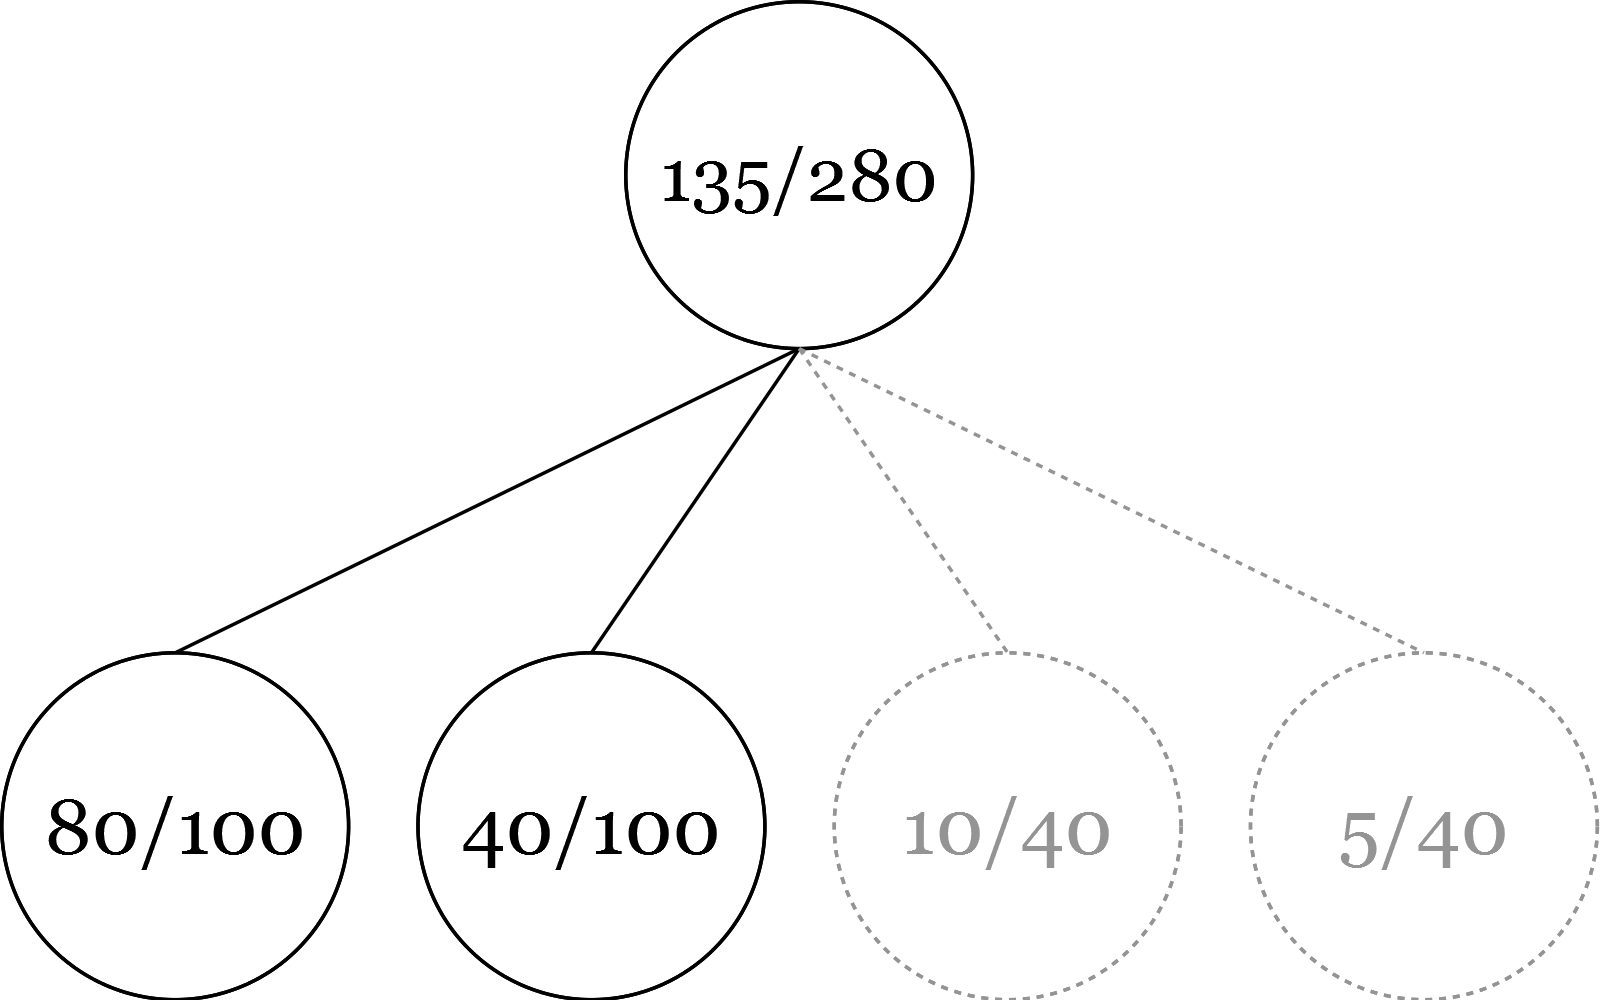
\includegraphics[width=.55\textwidth]{img/seq_halv_bp.png}
	\caption[Sequential Halving back-propagation example]{Average back-propagation and Sequential Halving example. The parent's value $0.48$, whereas the value of the best-reply is $0.8$.}
	\label{fig:seq_halv_bp}
\end{figure}

As an alternative to average back-propagation in the simple regret tree, \emph{maximum back-propagation} sets the value of each node to the maximum over their descendants. However, because nodes explored by Sequential Halving can only provide a recommendation at time $T$, the best node's intermediate values may be incorrect. Moreover, considering that the number of visits per ply declines proportional to the branching factor, deeper nodes that are sampled infrequently may only appear to have a good value due to insufficient sampling. Back-propagating such a node's value overrules many samples performed in the rest of the tree, disregarding many of the samples taken in potentially large sub-trees with higher confidence in their value.

The problem of back-propagation remains open. According to the theory, full exploration selection policies cannot give a recommendation at any time. However, in a tree, nodes' values should have a representative value at any time for UCT and Sequential Halving to be able to select promising nodes or sort nodes by value, respectively. In Section~\ref{sec:ulb_h-mcts}, an enhancement to Sequential Halving is discussed, which potentially reduces the number of suboptimal nodes sampled. As such, we can ensure that Sequential Halving converges to a best-reply over time.

\newpage
\section{Hybrid MCTS Solver}
\label{sec:hybmctssolver}

In the form presented in Algorithm~\ref{alg:h-mcts}, H-MCTS cannot solve proven wins or losses in the simple regret tree. Although we can employ the MCTS-Solver proposed by~\citeaby{Winands2008} in the UCT tree, the technique requires adaptation to Sequential Halving to be able to solve nodes in the simple regret tree. The main issue here is that when a solved child is encountered, the current round is interrupted to determine whether the node itself is solved as well. This leads to three different possible cases, in which this interruption can be encountered, and properly handled. Note that it is assumed that values are according to negamax, such that at each node, children's rewards are stored with respect to the player to move.
\begin{enumerate}
\item A solved win is encountered, in this case, we immediately want to remember this node and back-propagate to the parent. Any residual budget remains unspent in the current round.
\item A solved loss is encountered, but not all siblings lead to a loss. According to~\citeaby{Winands2008} it is appropriate in this case to count the visit as a loss. However, since there still exist nodes that do not lead to a loss, we have to ensure the solved node is not reselected. If it is reselected, a potentially high budget may be spent on the node, which results in an underestimation of the parent.
\item A solved loss is encountered, and all siblings lead to a loss. In this case the parent is a win and we should back-propagate immediately. Any residual budget remains unspent in the current round.
\end{enumerate}
\begin{figure}[hb]
	\centering
	\includegraphics[width=.6\textwidth]{img/solver.png}
	\caption[H-MCTS Solver example]{H-MCTS Solver removing a proven loss from selection. In the second round, node B is determined to be a proven loss, node C is returned to selection to fill the opened position.}
	\label{fig:h-mcts_solver}
\end{figure}

When running Sequential Halving, the first and last cases can be handled similar to the MCTS-Solver. The second case potentially leaves the assigned budget partially unspent. Because some children have been identified as a loss, while other unsolved options still remain, the proven losses should be removed from selection. Moreover, any budget left unspent due to this should be ``brought over'' to the next round, which starts with a reduced set of nodes. When a proven loss is discarded from selection, all children following this node move one position left, possibly returning an unsolved node to the current selection, as depicted in Figure~\ref{fig:h-mcts_solver}. If there is no unsolved node to return, the set of remaining arms is reduced after the round if it is smaller than $\ceil{\nicefrac{s}{2}}$, which means that more than half the nodes currently in $S_k$ were solved.

\IncMargin{1em}
\begin{algorithm2e}
\setstretch{1.0}
	\KwIn{node $p$, allocated budget $budget$}
	\KwOut{$t_p$: number of play-outs, $p1$ and $p2$ wins, solved player}
	\vspace{0.1cm}
	\func{h-mcts-solver}(node $p$, $budget$):										\;
	\Indp
	\lIf{isLeaf($p$)}{$I, S\gets$ \func{expand}($p$)}								\label{hs:children}
	$t_p \gets \tuple{0,0,0,0}$														\;		
	$b \gets \max{\left(1, \floor[\bigg]{\frac{p.budgetSpent + budget}{s\times\ceil{log_2{|S|}}}}\right)}$ \; 
	\If{$p$ is not root \textbf{and} $b < B $}{
		\For{i=0 \emph{\KwTo} budget}{
			$\tuple{v, w_1, w_2, s}_i \gets$ \func{uct-solver}($p$)						\;
			\func{update} $p, t_p$ with $\tuple{v, w_1,w_2, s}_i$							\;
		}
		\KwRet{$t_p$}
	}
	$b_u, k \gets 0$, $S_0 \gets S$, $s \gets |S_0|$\;
	\Repeat{$b_u \geq budget$ \textbf{or} $s < 2$} {														\label{hs:shot}
		$b_r \gets 0$																\; \label{hs:resid}
		\For{i=1 \emph{\KwTo} $s$}{
			$n_i \gets$ node $n$ at rank $i$ of $S_k$								\;
			\If{$n_i$ is not solved} {			
				\If{$b > n_i.visits$} {
					$b_i \gets b - n_i.visits$											\;
					\lIf{$i = 0$ \textbf{and} $s = 2$} { $b_i \gets \max{(b_i, budget - b_u - (b - n_1.visits))}$ }
					$b_i \gets \min{(b_i, budget - b_u)}$								\;
					$\tuple{v, w_1, w_2, s}_i \gets$ \func{h-mcts-solver}($n_i$, $b_i$)	\;
					\func{update} $p, b_u$, and $t_p$ with $\tuple{v, w_1, w_2, s}_i$		\;
				}
			}
			\uIf{$n_i$ is a win \textbf{or} $(n_i$ is a loss \textbf{and} $\forall n \in S: (n$ is a loss$))$}{
				set the solved player in $t_p$									\; \label{hs:solved}
				\func{update} $p.budgetSpent$ with $b_u$						\;
				\KwRet{$t_p$}													\;
			} \ElseIf{$(n_i$ is a loss \textbf{and} $\exists n \in S: (n$ is not a loss$))$}{
				$b_r \gets b_i - v$												\; \label{hs:update_resid}				
			}
			break if $b_u \geq budget$											\;
		}
		remove all solved nodes from $S$ and $S_k$								\;  \label{hs:remove}
		$k \gets k + 1$						\;
		$S_{k} \gets$ $S_{k-1}$, with the first $\max{(2, s)}$ elements sorted in descending order \; \label{hs:sort}
		$s \gets \ceil{\nicefrac{s}{2}}$										\;
		$s \gets \min{(s, |S|)}$												\; \label{hs:size_min}	
		\lIf{$s = 1$} {$b \gets b + (budget - b_u)$}
		\Else {	
			$b \gets b + \max{\left(1, \floor[\bigg]{\frac{p.budgetSpent + budget}{s\times\ceil{log_2{|S|}}}}\right)}$ \;
			$b \gets b + \ceil{\nicefrac{b_r}{s}}$														\; \label{hs:incr_budget_resid}
		}
	}
	\func{update} $p.budgetSpent$ with $b_u$										\;
	\Indm
	\KwRet{$t_p$}
  \caption{Hybrid Monte-Carlo Tree Search Solver (H-MCTS Solver). \label{alg:h-mcts-solver}}
\end{algorithm2e}
\DecMargin{1em}
\newpage
H-MCTS Solver is outlined in Algorithm~\ref{alg:h-mcts-solver}. The general procedure when a solved node is encountered is straightforward in the case of a solved win, and when all children are solved losses. The $budgetSpent$ is updated and the function immediately returns. The tuple $t_p$ now also contains a `solved' field, which holds the index of the player for which the node is solved. In this case the \func{update} function updates the node accordingly by setting the $isSolved$ flag. When an isolated proven loss is encountered, \ie not all siblings are losses, then we should not sample that node again, since it would under-evaluate the parent. This possibly leaves a residual budget $b_r$ declared on line~\ref{hs:resid}, which is maintained per round. When an isolated proven loss is found, the residual budget is updated on line~\ref{hs:update_resid} such that it can be spent in the next round with a reduced set of nodes, on line~\ref{hs:incr_budget_resid}. Moreover, since the isolated losses are removed from $S$ on line~\ref{hs:remove}, it is possible that $s > |S|$, which is restored on line~\ref{hs:size_min} after halving $s$. This ensures that previously removed nodes that were not proven losses can be returned to selection in case more than half of the nodes were solved in this round. On line~\ref{hs:sort} the set of children from the previous round $S_{k-1}$ is sorted, as such $|S_k| = |S|$ for each round. Therefore, when a solved loss is removed from selection, another child can take its place. Note also that on line~\ref{hs:children}, a second set $I$ contains all children. Because it is possible to remove all nodes from $S$ in case of a proven loss, $I$ is never altered and can be used to give a recommendation at the root.

\section{Upper and Lower Bounds for H-MCTS}
\label{sec:ulb_h-mcts}
A disadvantage of Sequential Halving applied to game trees is that nodes that can never improve on the current best reply are sampled relatively frequently. Although this is theoretically sound in providing lower guarantees on simple regret, practically it means that nodes are often sampled when it is clearly futile to do so. 

For example, consider a set of 5 nodes $S_1$, in which there exists one node with a true mean $\mu^*$ of $0.7$, all other nodes have means of $-0.5$. Only a few samples are required to find out which node is the best reply. However, as shown in the example in Figure~\ref{fig:seq-halving}, the second-best node are sampled as often as the best one, and in effect the parent's value is underestimated. 

To counter this problem we can compare a child's upper confidence bound to its best sibling's lower confidence bound. In this optimistic scheme it is assumed that a node can still improve its value such that it becomes better than the current best reply, if their respective upper and lower confidence bounds overlap. Recall from Chapter~\ref{chap:mab}, that the upper confidence bound represents the highest value a node can achieve with overwhelming probability. This approach can be inverted to acquire the lowest possible value a node is likely to achieve,
\begin{equation}
  	v_i - C \times \displaystyle\sqrt{\frac{\ln{n_p}}{n_i}}.
\end{equation}
Because a sorted list of children is maintained in the simple regret tree, the best child's bound can be compared to it siblings' bounds at any time. Therefore, when selecting a node to be investigated, only if the current node's upper confidence bound overlaps with the currently estimated best-reply's lower confidence bound, should we assume that it is still possible for this node to improve upon the current best node's score. As such we can skip any node with a non-overlapping bound with the best node. This potentially saves a substantial budget which would otherwise have been spent sampling suboptimal nodes. An example of this enhancement is depicted in Figure \ref{fig:ublb}. In this example, the current best node's lower bound overlaps only with the upper bounds of nodes $B$ and $C$.

\begin{figure}[b]
	\centering
	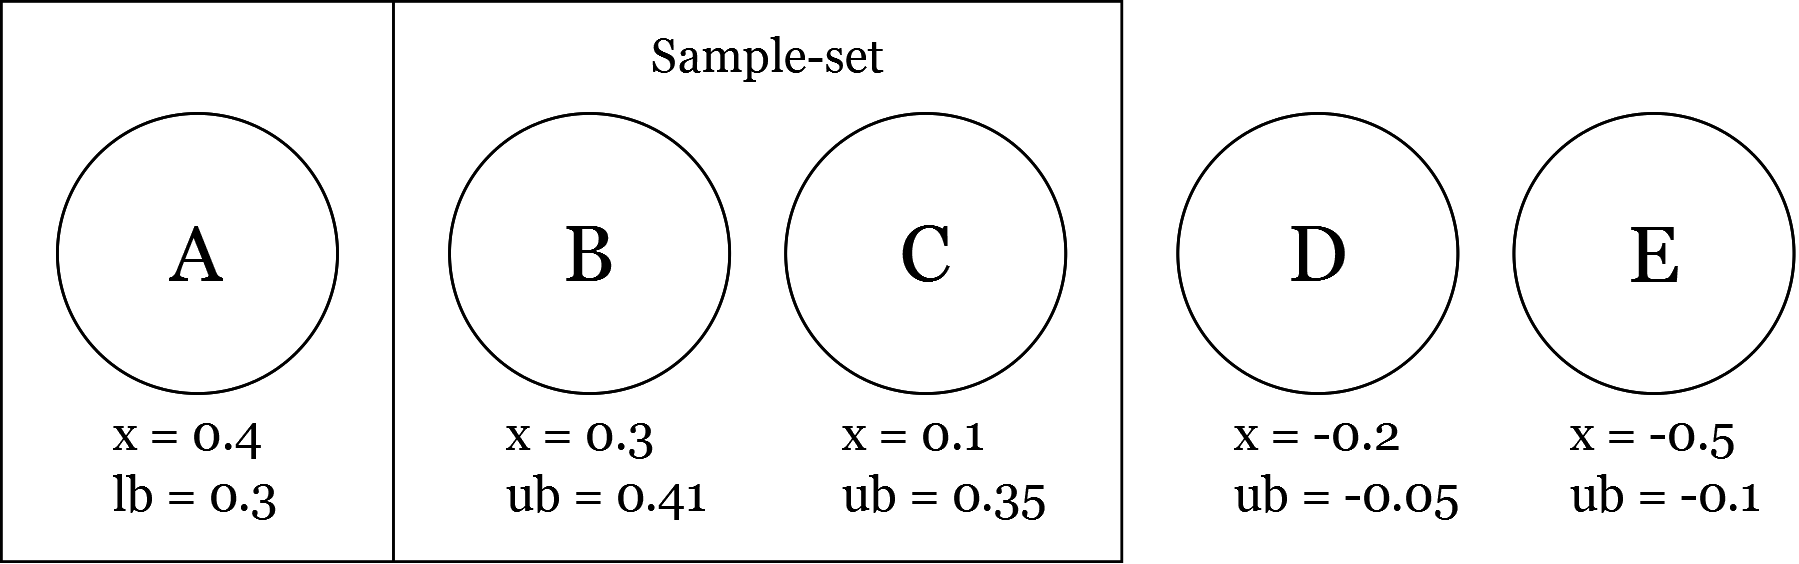
\includegraphics[width=.55\textwidth]{img/ublb.png}
	\caption[Upper/Lower Bound enhancement example]{Example upper/lower bound Sequential Halving. Node A is the current empirical best, with a lower confidence bound of $0.1$. Only nodes B and C have upper confidence bounds that overlap with this lower bound. D and E are not sampled this round.}
	\label{fig:ublb}
\end{figure}

\IncMargin{1em}
\begin{algorithm2e}
\setstretch{0.9}
	\KwIn{node $p$, allocated budget $budget$}
	\KwOut{$t_p$: number of play-outs, $p1$ and $p2$ wins, solved player}
	\vspace{0.1cm}
	\func{h-mcts-solver}(node $p$, $budget$):										\;
	\Indp
	\lIf{isLeaf($p$)}{$I, S\gets$ \func{expand}($p$)}					
	$t_p \gets \tuple{0,0,0,0}$														\;		
	$b \gets \max{\left(1, \floor[\bigg]{\frac{p.budgetSpent + budget}{s\times\ceil{log_2{|S|}}}}\right)}$ \; 
	\If{$p$ is not root \textbf{and} $b < B $}{
		\For{i=0 \emph{\KwTo} budget}{
			$\tuple{v, w_1, w_2, s}_i \gets$ \func{uct-solver}($p$)						\;
			\func{update} $p, t_p$ with $\tuple{v, w_1,w_2, s}_i$							\;
		}
		\KwRet{$t_p$}
	}
	$b_u, k \gets 0$, $S_0 \gets S$, $s \gets |S_0|$\;
	\Repeat{$b_u \geq budget$ \textbf{or} $s < 2$} {
		$b_r \gets 0$																\;
		\For{i=1 \emph{\KwTo} $\min{(s,|S_k|)}$}{
			$n_i \gets$ node $n$ at rank $i$ of $S_k$								\;
			\If{$n_i$ is not solved} {			
				\If{$b > n_i.visits$} {
					$b_i \gets b - n_i.visits$											\;
					\lIf{$i = 0$ \textbf{and} $s = 2$} { $b_i \gets \max{(b_i, budget - b_u - (b - n_1.visits))}$ }
					$b_i \gets \min{(b_i, budget - b_u)}$								\;
					\If {$i > 0$ \textbf{and} $n_i.value + C \times \sqrt{\frac{\ln{p.visits}}{n_i.visits}} < l_b$} { \label{ublb:upper_bound}
						$b_r \gets b_r + b_i$ \;									
						\textbf{continue}	\;	\label{ublb:skip}
					}
					$\tuple{v, w_1, w_2, s}_i \gets$ \func{h-mcts-solver}($n_i$, $b_i$)	\;
					\func{update} $p, b_u$, and $t_p$ with $\tuple{v, w_1, w_2, s}_i$		\;
					\lIf{$i = 0$} {$l_b \gets n_i.value - C \times \sqrt{\frac{\ln{p.visits}}{n_i.visits}}$} \label{ublb:lower_bound}
				}
			}
			\uIf{$n_i$ is a win \textbf{or} $(n_i$ is a loss \textbf{and} $\forall n \in S: (n$ is a loss$))$}{
				set the solved player in $t_p$									\;
				\func{update} $p.budgetSpent$ with $b_u$						\;
				\KwRet{$t_p$}													\;
			} \ElseIf{$(n_i$ is a loss \textbf{and} $\exists n \in S: (n$ is not a loss$))$}{				
				$b_r \gets b_i - v$												\;				
			}
			break if $b_u \geq budget$											\;
		}
		remove all solved nodes from $S$ and $S_k$								\;
		$k \gets k + 1$															\;
		$S_{k} \gets$ $S_{k-1}$, with the first $\max{(2, s)}$ elements sorted in descending order					\;
		$s \gets \ceil{\nicefrac{s}{2}}$									\;
		$s \gets \min{(s, |S|)}$												\;
		\lIf{$s = 1$} {$b \gets b + (budget - b_u)$}
		\Else{
			$b \gets b + \max{\left(1, \floor[\bigg]{\frac{p.budgetSpent + budget}{s\times\ceil{log_2{|S|}}}}\right)}$ \;
			$b \gets b + \ceil{\nicefrac{b_r}{s}}$\;	\label{ublb:reallo}
		}
	}
	\func{update} $p.budgetSpent$ with $b_u$										\;
	\Indm
	\KwRet{$t_p$}
  \caption{Hybrid Monte-Carlo Tree Search Solver with Overlapping Bounds. \label{alg:h-mcts-ublb}}
\end{algorithm2e}
\DecMargin{1em}

This enhancement also ensures that over time Sequential Halving samples greedily. Given infinite samples, the lower and upper confidence bounds of two nodes should only ever overlap if they have the same value. Since, in this case only the nodes with the highest averages are sampled, Sequential Halving with the Upper/Lower Bounds enhancement tends to sample only the best node(s) over time.

The Overlapping Bounds enhancement for H-MCTS is detailed in Algorithm~\ref{alg:h-mcts-ublb}, in which it is combined with the solver discussed in the previous subsection. On line~\ref{ublb:lower_bound} the lower confidence bound of the current best node is determined. Note that this is performed in each round, right after the best node of the round is sampled. This ensures that we have the best estimate for the current lower bound. All other children's upper confidence bounds are then compared to the current best lower bound on line~\ref{ublb:upper_bound}. If the bounds do not overlap, the node is skipped, line~\ref{ublb:skip}. Similar to the solver, the unspent budget is reserved in $b_r$, it is reallocated on line~\ref{ublb:reallo} to be spent in the next round.

% -------------------------------------------------------------------------------
% ------------------- ::::::: Experiments and Results ::::::: -------------------
% -------------------------------------------------------------------------------
\chapter{Experiments and Results}
\label{chap:experiments}
\begin{chaptercontents}
H-MCTS is thoroughly evaluated in six distinct two-player games: Amazons, AtariGo, Ataxx, Breakthrough, NoGo, and Pentalath.
\end{chaptercontents}

\section{Experimental Setup}
\label{sec:ex_setup}
In this chapter the results of the experiments performed on six two-player games are presented. H-MCTS and the games were implemented in two different engines. Amazons, Breakthrough, NoGo, and Pentalath are implemented in a Java based engine. Ataxx and AtariGo are implemented in a \emph{C++} based engine.\footnote{Experiments in Ataxx and AtariGo were performed in collaboration with Prof. Dr. Tristan Cazenave.} Whereas the former is a full implementation of SHOT, H-MCTS, H-MCTS Solver, and the Upper/Lower Bounds enhancement, the latter consists of an implementation of SHOT and H-MCTS.

A brief description of each game is given below:
\begin{itemize}
\item \emph{Amazons} is played on a 10$\times$10 chessboard. Players each have four Amazons that move as queens in chess. Moves consist of two parts, movement, and shooting an arrow to block a square on the board. The last player to move wins the game.
\item \emph{AtariGo}, or first-capture Go, is a variant of Go where the first player to capture any stones wins. The experiments are performed on a 9$\times$9 board.
\item \emph{Ataxx} is a game similar to Reversi. Played on a square board, players start with two stones each placed in an opposite corner. Captures are performed by moving a stone alongside an opponent's on the board. In the variant used in this thesis, jumps are not allowed. The game ends when all squares are filled, or when a player has no remaining stones. The player with the most stones wins.  The experiments are performed on a 7$\times$7 board.
\item \emph{Breakthrough} is played on an 8$\times$8 board. Players start with 16 pawns. The goal is to move one of them to the opponent's side.
\item \emph{NoGo} is a combinatorial game based on Go. Captures are forbidden and the first player unable to play due to this rule, loses. The experiments are performed on a 9$\times$9 board.
\item \emph{Pentalath} is a connection game played on a hexagonal board. The goal is to place 5 pieces in a row. Pieces can be captured by fully surrounding an opponent's set of pieces.
\end{itemize}

All games use a uniform random selection policy during the play-outs, unless otherwise stated. All algorithms use transposition tables to store the values of game-states, these tables are cleared between moves, such that no information is retained. The $C$ constant, used by UCT (Equation \ref{eq:uct}) was optimized for each game and was not re-optimized for H-MCTS, unless mentioned otherwise, both UCT and H-MCTS use the same $C$ constant. Table~\ref{tab:uct_c} lists the $C$ constant used by UCT and H-MCTS in the experiments in this section.

\begin{table}[ht]
\centering
\captionsetup{justification=centering,margin=1cm}
\tabcolsep=0.45cm
\scalebox{0.9}{
\begin{tabular}{r|l}
\hline
\textbf{Game} & \multicolumn{1}{c}{$C$ Constant}  \\ [1mm] 
\cline{1-2}
\multicolumn{1}{c|}{} & \multicolumn{1}{c}{} \\ [-3mm]
Amazons 			    	& 0.4 	\\ [.5mm] 
AtariGo 9$\times$9  		& 0.125	\\ [.5mm] 
Ataxx 7$\times$7  			& 0.5	\\ [.5mm] 
Breakthrough 8$\times$8 	& 0.8	\\ [.5mm] 
NoGo 9$\times$9  			& 0.6	\\ [.5mm] 
Pentalath 		  			& 0.8 	\\ [.5mm] 
\hline
\end{tabular}
}
\vspace{3mm}
{\caption{$C$ Constants used by H-MCTS and UCT.} \label{tab:uct_c}}
\end{table}

Because H-MCTS cannot be terminated any time we present only results for a fixed number of simulations. In each experiment, both players are allocated a budget of both 10,000 and 25,000 play-outs.
\newpage
\section{Results}
\label{sec:results}
For the tables and graphs in this section, results are shown with respect to the first algorithm mentioned in the captions, along with a 95\% confidence interval. For each experiment, the players' seats were swapped such that 50\% of the games are played as the first player, and 50\% as the second, to ensure no first-player or second-player bias.

This section is structured as follows: first, in Subsection \ref{subsec:shot_uct} the performance of SHOT is compared to UCT. Followed by the results of games played by H-MCST against UCT in Subsection \ref{subsec:hmcts_uct}. The results presented in these subsections form the baseline for the experiments in the following ones. First, to determine the influence of UCT in H-MCTS, Subsection~\ref{subsec:hmcts_shot} details the results of games played by H-MCTS against SHOT. Followed by a detailed investigation into the performance of the H-MCTS Solver in Subsection~\ref{subsec:hmcts_solver}. Finally, the performance of the Upper/Lower Bounds enhancement for H-MCTS is investigated in Subsection~\ref{subsec:hmcts_ublb}. Finally, Subsection~\ref{subsubsec:h-mcts_c} explores the influence of the $C$ constant in H-MCTS.

\subsection{SHOT and UCT}
\label{subsec:shot_uct}

SHOT is the algorithm used in H-MCTS' simple regret tree, thus SHOT can be considered an instance of H-MCTS when $B = 0$. In this subsection SHOT is compared to UCT to determine a baseline for the H-MCTS experiments.

\begin{table}[ht]
\centering
\captionsetup{justification=centering,margin=1cm}
\tabcolsep=0.45cm
\scalebox{0.89}{
\begin{tabular}{r|ll}
\hline
 & \multicolumn{1}{c}{\textbf{10,000}} & \multicolumn{1}{c}{\textbf{25,000}} \\ 
\textbf{Game} & \multicolumn{1}{c}{\textbf{play-outs}} & \multicolumn{1}{c}{\textbf{play-outs}} \\ [1mm] 
\cline{1-3}
\multicolumn{1}{c|}{} & \multicolumn{2}{c}{} \\ [-3mm]
Amazons 			    	& {\bf{60.2}} $\pm$ 3.0 	& {\bf{55.2}} $\pm$ 3.1 	\\ [.5mm] 
AtariGo 9$\times$9  		& {\bf{53.8}} $\pm$ 3.1 	& {\bf{55.7}} $\pm$ 3.1 	\\ [.5mm] 
Ataxx 7$\times$7  			& 46.7 $\pm$ 3.1			& 40.8 $\pm$ 3.1 			\\ [.5mm] 
Breakthrough 8$\times$8 	& 31.2 $\pm$ 3.1			& 16.4 $\pm$ 2.3 			\\ [.5mm] 
NoGo 9$\times$9  			& 44.7 $\pm$ 3.1 			& 41.4 $\pm$ 3.1 			\\ [.5mm] 
Pentalath 		  			& 33.7 $\pm$ 3.0 			& 22.8 $\pm$ 2.6 			\\ [.5mm] 
\hline
\end{tabular}
}
\vspace{3mm}
{\caption[SHOT vs. UCT.]{SHOT vs. UCT, random play-outs\\ Win percentages with respect to SHOT. 1,000 games} \label{tab:uct_phot}}
\end{table}

SHOT played 1,000 matches against UCT per game, for each budget setting, results are shown in Table~\ref{tab:uct_phot}. SHOT performs best in the games with the highest branching factors, Amazons, AtariGo and to a lesser extent in NoGo. The NoGo results differ from those presented in~\citebay{Cazenave14SHOT} because this experiment is run using a fixed allocation of play-outs for both algorithms, unlike the experiments performed by Cazenave where SHOT receives a fixed budget, and UCT is allocated SHOT measured running time. The results reinforce the evidence that Sequential Halving is best applied in games with high branching factors. In the games with narrow winning-lines such as Breakthrough and Pentalath, SHOT's performance declines significantly against UCT. However, given SHOT's speed improvement over UCT, it is possible that the technique performs better in a time-based experiment.

\subsection{H-MCTS and UCT}
\label{subsec:hmcts_uct}

In this subsection, experiments comparing H-MCTS to UCT are detailed. Considering that H-MCTS uses UCT when a small budget is available, the benefit of minimizing simple regret near the root is determined by performing experiments where H-MCTS plays against UCT.

\begin{figure}[ht]
\centering
\captionsetup{justification=centering,margin=1cm}
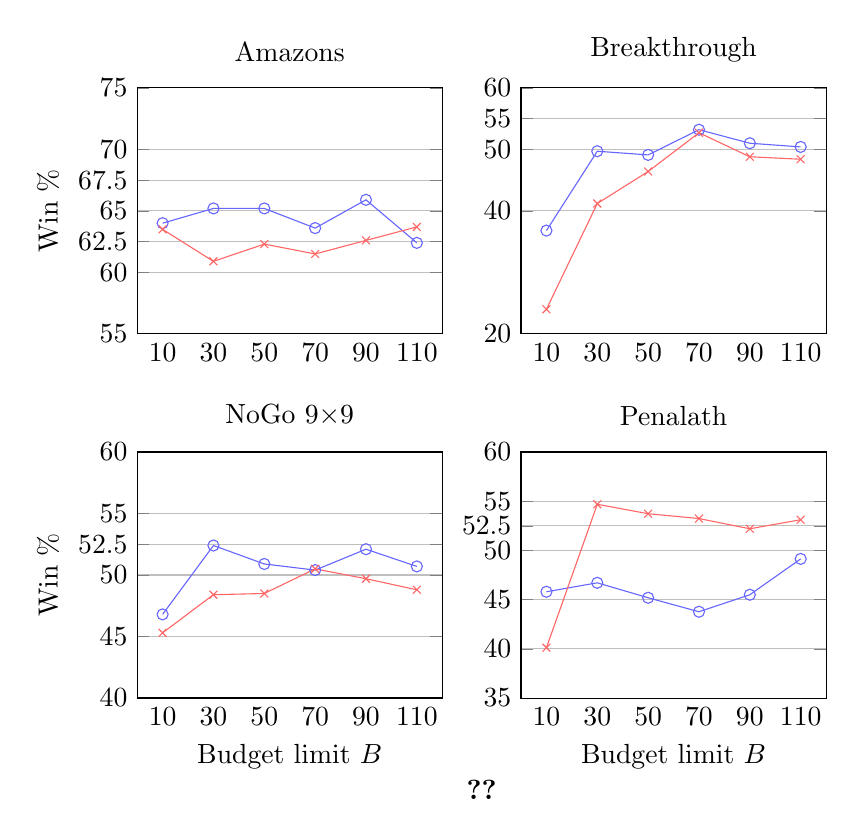
\begin{tikzpicture}
\begin{groupplot}
    [
        group style=
            {
            columns=2,
            rows=2,
            xlabels at=edge bottom,
            ylabels at=edge left,
            vertical sep= 1.5cm,
            },
        legend columns=2,
       	width  = 0.45*\textwidth,
        major x tick style = transparent,
        %ybar= 2 * \pgflinewidth,
        % bar width = 10pt,
        ymajorgrids = true,
        ylabel = {Win \%},
        xlabel= {Budget limit $B$},
        symbolic x coords={10,30,50,70,90,110},
        xtick = data,
        ytick={0,20,30,40,45,50,55,60,65,70,80},
        scaled y ticks = false,
        enlarge x limits = 0.1,
        ymin=0, ymax=80
    ]
% Amazons ----------------------------------------
\nextgroupplot[title=Amazons, ymin=55, ymax=75, ytick={55,60,62.5,65,67.5,70,75}]
\addplot[blue!60!white, mark=o, range=50:70]
	coordinates {(10, 64) +- (0,2.98) 
	(30,65.2) +- (0,2.95)
	(50,65.2) +- (0,2.95)
	(70,63.6) +- (0,2.98)
	(90,65.9) +- (0,2.94)
	(110,62.4) +- (0,3.00)};
\addplot[red!60!white, mark=x]
	coordinates {(10,63.5) +- (0,2.98)
	(30,60.9) +- (0,3.02)
	(50,62.3) +- (0,3.00)
	(70,61.5) +- (0,3.02)
	(90,62.6) +- (0,3.00)
	(110,63.7)+- (0,2.98)};
% Breakthrough -------------------------------------
\nextgroupplot[title=Breakthrough, ymin=20, ymax=60, ytick={20,40,50,55,60}]
\addplot[blue!60!white, mark=o]
	coordinates {(10, 36.8) +- (0,2.99) 
	(30,49.7) +- (0,3.1)
	(50,49.1) +- (0,3.1)
	(70,53.2) +- (0,3.1)
	(90,51) +- (0,3.1)
	(110,50.4) +- (0,3.1)};
\addplot[red!60!white, mark=x]
	coordinates {(10,24) +- (0,2.65)
	(30,41.2) +- (0,3.05)
	(50,46.4) +- (0,3.09)
	(70,52.7) +- (0,3.09)
	(90,48.8) +- (0,3.10)
	(110,48.4)+- (0,3.10)};
% NoGo --------------------------------------------
\nextgroupplot[title=NoGo 9$\times$9, ymin=40, ymax=60, ytick={20,40,45,50,52.5,55,60}]
\addplot[blue!60!white, mark=o]
	coordinates {(10, 46.8) +- (0,3.09) 
	(30,52.4) +- (0,3.1)
	(50,50.9) +- (0,3.1)
	(70,50.4) +- (0,3.1)
	(90,52.1) +- (0,3.1)
	(110,50.7) +- (0,3.1)};
\addplot[red!60!white, mark=x]
	coordinates {(10,45.3) +- (0,3.09)
	(30,48.4) +- (0,3.1)
	(50,48.5) +- (0,3.1)
	(70,50.5) +- (0,3.1)
	(90,49.7) +- (0,3.1)
	(110,48.8)+- (0,3.1)};

% Pentalath --------------------------------------------
\nextgroupplot[title=Penalath, legend to name=grouplegend, ymin=35, ymax=60, ytick={20,35,40,45,50,52.5,55,60}]
\addplot[blue!60!white, mark=o]
	coordinates {(10, 45.8) +- (0,3.11) 
	(30,46.71) +- (0,3.11)
	(50,45.19) +- (0,3.11)
	(70,43.77) +- (0,3.1)
	(90,45.5) +- (0,3.1)
	(110,49.14) +- (0,3.1)};
	\addlegendentry{10,000 play-outs}
\addplot[red!60!white, mark=x]
	coordinates {(10,40.12) +- (0,3.07)
	(30,54.69) +- (0,3.12)
	(50,53.73) +- (0,3.14)
	(70,53.24) +- (0,3.12)
	(90,52.2) +- (0,3.13)
	(110,53.12)+- (0,3.13)};
	\addlegendentry{25,000 play-outs}
\end{groupplot}

    \node (legend) at ($(group c1r2.south)!0.5!(group c2r2.south)$)
      [below, yshift=-2\pgfkeysvalueof{/pgfplots/every axis title shift}]
      {\ref{grouplegend}};

\end{tikzpicture}
     \caption[H-MCTS $B$ values]{H-MCTS vs. UCT, random play-outs. \\ Win percentages with respect to H-MCTS. 1,000 games per data point.}
     \label{fig:h-mcts_v_uct}
\end{figure}



Figure~\ref{fig:h-mcts_v_uct} gives an overview of the results for different budget limits $B$ in H-MCTS. For each game 1,000 matches were played with a budget of 10,000 and 25,000 play-outs against UCT. 

For Amazons, different settings of $B$ do not significantly influence the performance of H-MCTS, H-MCTS performs consistently better than UCT in this domain. This is mainly due to the large branching factor of approximately $1,200$ moves at the start of the match. In this case, UCT spreads its budget out, allocating it almost randomly because it is unable to procure sufficient visits per move to decrease their confidence bounds. Unlike UCT though, H-MCTS initially performs several rounds with a large set of options, but reduces the number of nodes under consideration quickly, allowing it to focus on a subset of moves found to be promising. 

Mainly in Breakthrough and Pentalath does the value of $B$ have an impact on performance. In Pentalath the graphs show evidence that an increase in performance may be obtained given a larger budget of play-outs. For NoGo, the trend is similar to Amazons', the value of $B$ has no large influence on performance. The graphs show that the best budget limit per game does not change significantly when the algorithm is given a higher deliberation time. 

\begin{table}[t]
\centering
\captionsetup{justification=centering,margin=1cm}
\tabcolsep=0.3cm
\scalebox{1.0}{
\begin{tabular}{rlll}
\hline
\multicolumn{2}{c|}{} & \multicolumn{1}{c}{\textbf{10,000}} & \multicolumn{1}{c}{\textbf{25,000}} \\ 
\textbf{Game} & \multicolumn{1}{c|}{\textbf{$B$}} & \multicolumn{1}{c}{\textbf{play-outs}} & \multicolumn{1}{c}{\textbf{play-outs}} \\ [1mm] 
\cline{1-4}
\multicolumn{2}{c|}{} \\ [-3mm]
Amazons &\multicolumn{1}{l|}{90}			    	& {\bf{64.3}} $\pm$ 2.1 		& {\bf{64.3}} $\pm$ 2.1 		\\ [.5mm] 
Breakthrough 8$\times$8 &\multicolumn{1}{l|}{70}	& 51.8 $\pm$ 2.2				& 47.7 $\pm$ 2.2 				\\ [.5mm] 
NoGo 9$\times$9 &\multicolumn{1}{l|}{30} 			& 49.9 $\pm$ 2.2				& 48.3 $\pm$ 2.2 				\\ [.5mm] 
Pentalath &\multicolumn{1}{l|}{30} 		  			& 46.6 $\pm$ 2.2				& 51.7 $\pm$ 2.2 				\\ [.5mm] 
\hline
\end{tabular}
}
\vspace{3mm}
{\caption[H-MCTS vs. UCT.]{H-MCTS vs. UCT, random play-outs.\\ Win percentages with respect to H-MCTS. 2,000 games} \label{tab:uct_hmcts}}
\end{table}

\begin{table}[t]
\centering
\captionsetup{justification=centering,margin=1cm}
\tabcolsep=0.3cm
\scalebox{1.0}{
\begin{tabular}{rlll}
\hline
\multicolumn{2}{c|}{} & \multicolumn{1}{c}{\textbf{10,000}} & \multicolumn{1}{c}{\textbf{25,000}} \\ 
\textbf{Game} & \multicolumn{1}{c|}{\textbf{$B$}} & \multicolumn{1}{c}{\textbf{play-outs}} & \multicolumn{1}{c}{\textbf{play-outs}} \\ [1mm] 
\cline{1-4}
\multicolumn{2}{c|}{} \\ [-3mm]
AtariGo 9$\times$9 &\multicolumn{1}{l|}{30} 		& {\bf{57.9}} $\pm$ 3.1 	& {\bf{69.1}} $\pm$ 2.9 		\\ [.5mm] 
Ataxx 7$\times$7 &\multicolumn{1}{l|}{30} 			& 52.5 $\pm$ 3.1			& {\bf{65.2}} $\pm$ 3.0 		\\ [.5mm] 
\hline
\end{tabular}
}
\vspace{3mm}
{\caption[H-MCTS vs. UCT (Ataxx and AtariGo)]{H-MCTS vs. UCT, random play-outs.\\ Win percentages with respect to H-MCTS. 1,000 games} \label{tab:uct_hmcts_tristan}}
\end{table}

The best results for the values of $B$ from Figure~\ref{fig:h-mcts_v_uct} were used to run an additional 1,000 matches per game, of which the results are presented in Table~\ref{tab:uct_hmcts}. The best $B$ for either 10,000 or 25,000 play-outs is selected based on the highest win-rate achieved. Results for 1,000 games in AtariGo and Ataxx are shown in Table~\ref{tab:uct_hmcts_tristan}. A significant performance increase for H-MCTS in both games is revealed in these games. 

H-MCTS performs best in Amazons, Ataxx, and AtariGo. In Pentalath, given a higher total budget there is evidence that performance increases. To validate this conjecture in Pentalath, an additional 1,000 games were played with a budget of 50,000 play-outs. This resulted in a win-rate for H-MCTS of {\bf{55.0}}\%$\pm$3.1, a significant increase in performance over both UCT, and the 25,000 play-out case.

In Breakthrough, performance drops significantly given a higher overall budget. This may be due to the fact that the game has narrow winning-lines, and a more exploiting algorithm works better by identifying promising moves and exploiting them rapidly. Moreover, in this experiment both techniques use a random play-out policy. This means that because the results returned by these play-outs are less trustworthy, it is likely that Sequential Halving excludes a good move from selection too soon. This has a potentially large impact on performance, because moves that have been removed from selection cannot be re-selected at the root, and will therefore never be recommended.

Note that it is possible that H-MCTS requires separate tuning of its UCT $C$ constant in games. This optimization was performed for Ataxx and AtariGo, which resulted in winning rates for H-MCTS of {\bf{61.7}}\%$\pm$3.0, and {\bf{66.6}}\%$\pm$3.0 in AtariGo with a $C$ constant of $0.25$, and {\bf{57.6}}\%$\pm$3.1, and {\bf{58.1}}\%$\pm$3.1 in Ataxx with a $C$ constant of $0.125$, for 10,000 and 25,000 play-outs, respectively.

\subsection{H-MCTS and SHOT}
\label{subsec:hmcts_shot}

\begin{table}[t]
\centering
\captionsetup{justification=centering,margin=1cm}
\tabcolsep=0.3cm
\scalebox{1.0}{
\begin{tabular}{rlll}
\hline
\multicolumn{2}{c|}{} & \multicolumn{1}{c}{\textbf{10,000}} & \multicolumn{1}{c}{\textbf{25,000}} \\ 
\textbf{Game} & \multicolumn{1}{c|}{\textbf{$B$}} & \multicolumn{1}{c}{\textbf{play-outs}} & \multicolumn{1}{c}{\textbf{play-outs}} \\ [1mm] 
\cline{1-4}
\multicolumn{2}{c|}{} \\ [-3mm]
Amazons &\multicolumn{1}{l|}{50}			    	& 51.2 $\pm$ 3.1 			& {\bf{55.4}} $\pm$ 3.1 	\\ [.5mm] 
AtariGo 9$\times$9 &\multicolumn{1}{l|}{30} 		& {\bf{53.2}} $\pm$ 3.1 	& {\bf{61.2}} $\pm$ 3.0		\\ [.5mm] 
Ataxx 7$\times$7 &\multicolumn{1}{l|}{30} 			& {\bf{55.2}} $\pm$ 3.1		& {\bf{65.3}} $\pm$ 3.0 	\\ [.5mm] 
Breakthrough 8$\times$8 &\multicolumn{1}{l|}{70}	& {\bf{68.4}} $\pm$ 2.9  	& {\bf{84.0}} $\pm$ 2.3 	\\ [.5mm] 
NoGo 9$\times$9 &\multicolumn{1}{l|}{30} 			& {\bf{56.3}} $\pm$ 3.1 	& {\bf{55.5}} $\pm$ 3.1 	\\ [.5mm] 
Pentalath &\multicolumn{1}{l|}{30} 		  			& {\bf{62.1}} $\pm$ 3.0		& {\bf{78.3}} $\pm$ 2.6  	\\ [.5mm] 
\hline
\end{tabular}
}
\vspace{3mm}
{\caption[H-MCTS vs. SHOT.]{H-MCTS vs. SHOT, random play-outs\\ Win percentages with respect to H-MCTS. 1,000 games} \label{tab:shot_hmcts}}
\end{table}

To determine the effect of UCT in H-MCTS, the results of matches played against SHOT are shown in Table~\ref{tab:shot_hmcts}. H-MCTS shows significant improvement in 10 of the 12 cases. No use is made of the speed benefits of either technique in these experiments. 

These results give evidence for the claim that H-MCTS makes use of UCT's any time property to provide proper utility estimates in the simple regret tree. Values back-propagated by UCT may be more effective than those back-propagated by using Sequential Halving throughout the tree. Because H-MCTS also performs better than SHOT against UCT in these games, H-MCTS likely performs better in general than SHOT given a fixed play-out budget.
\newpage
\subsection{H-MCTS Solver}
\label{subsec:hmcts_solver}

In this subsection, the influence of the solver enhancement in H-MCTS and SHOT is investigated. Experiments are performed to show the performance of the solver per technique individually, and for H-MCTS against UCT.

\begin{figure}[h]
\centering
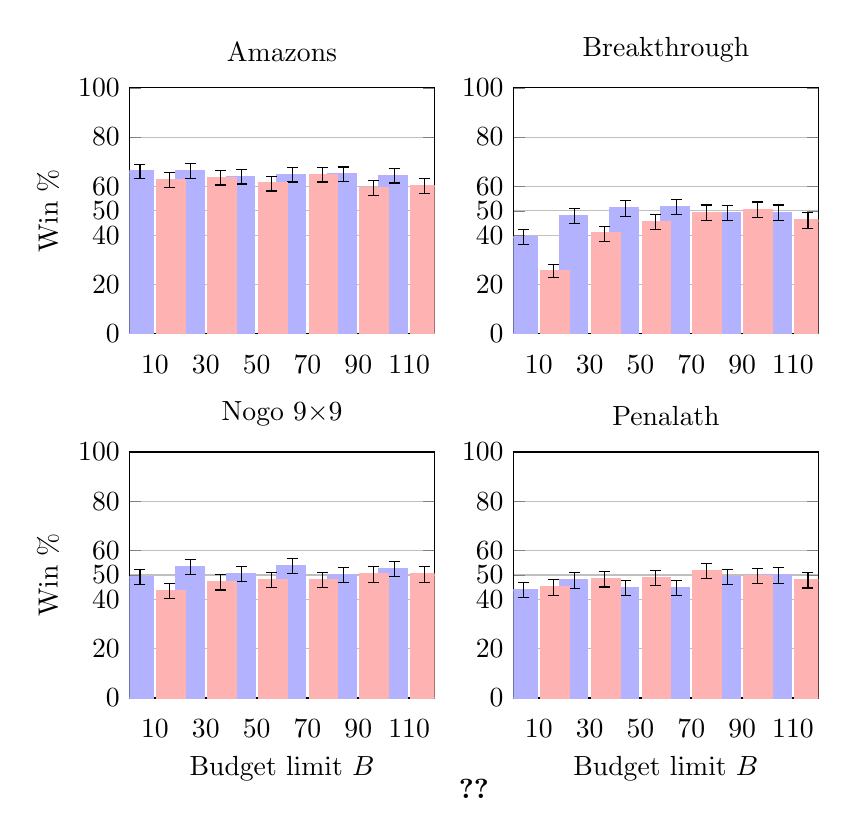
\begin{tikzpicture}
\begin{groupplot}
    [
        group style=
            {
            columns=2,
            rows=2,
            xlabels at=edge bottom,
            ylabels at=edge left,
            vertical sep= 1.5cm,
            },
       	width  = 0.45*\textwidth,
        major x tick style = transparent,
        ybar= 2 * \pgflinewidth,
        % bar width = 10pt,
        ymajorgrids = true,
        ylabel = {Win \%},
        xlabel= {Budget limit $B$},
        symbolic x coords={10,30,50,70,90,110},
        xtick = data,
        ytick={0,20,40,50, 60,80,100},
        scaled y ticks = false,
        enlarge x limits = 0.1,
        ymin=0,
        ymax=100,
    ]
% Amazons ----------------------------------------
\nextgroupplot[title=Amazons]
\addplot[blue!30!white, fill=blue!30!white, thick, error bars/.cd,
            y dir=both, error bar style={black},
            y explicit]
	coordinates {
	(10, 66) +- (0,2.94) 
	(30,66.2) +- (0,2.93)
	(50,63.9) +- (0,2.98)
	(70,64.7) +- (0,2.96)
	(90,64.9) +- (0,2.96)
	(110,64.3) +- (0,2.97)};
\addplot[red!30!white, fill=red!30!white, thick, error bars/.cd,
            y dir=both, error bar style={black},
            y explicit]
	coordinates {
	(10,62.6) +- (0,3)
	(30,63.5) +- (0,2.99)
	(50,61.1) +- (0,3.02)
	(70,64.7) +- (0,2.96)
	(90,59.3) +- (0,3.04)
	(110,60.1)+- (0,3.04)};
% Breakthrough -------------------------------------
\nextgroupplot[title=Breakthrough]
\addplot[blue!30!white, fill=blue!30!white, thick, error bars/.cd,
            y dir=both, error bar style={black},
            y explicit]
	coordinates {
	(10, 39.48) +- (0,3.03) 
	(30,47.8) +- (0,3.1)
	(50,50.95) +- (0,3.1)
	(70,51.6) +- (0,3.1)
	(90,49.2) +- (0,3.1)
	(110,49.3) +- (0,3.1)};
\addplot[red!30!white, fill=red!30!white, thick, error bars/.cd,
            y dir=both, error bar style={black},
            y explicit]
	coordinates {
	(10,25.45) +- (0,2.7)
	(30,40.78) +- (0,3.05)
	(50,45.35) +- (0,3.09)
	(70,49.3) +- (0,3.1)
	(90,50.5) +- (0,3.1)
	(110,46.1)+- (0,3.09)};
% Nogo --------------------------------------------
\nextgroupplot[title=Nogo 9$\times$9]
\addplot[blue!30!white, fill=blue!30!white, thick, error bars/.cd,
            y dir=both, error bar style={black},
            y explicit]
	coordinates {
	(10, 49.3) +- (0,3.1) 
	(30,53.3) +- (0,3.09)
	(50,50.4) +- (0,3.1)
	(70,53.6) +- (0,3.09)
	(90,50.0) +- (0,3.1)
	(110,52.5) +- (0,3.1)};
\addplot[red!30!white, fill=red!30!white, thick, error bars/.cd,
            y dir=both, error bar style={black},
            y explicit]
	coordinates {
	(10,43.6) +- (0,3.07)
	(30,47) +- (0,3.09)
	(50,48) +- (0,3.1)
	(70,48) +- (0,3.1)
	(90,50.2) +- (0,3.1)
	(110,50.2)+- (0,3.1)};

% Pentalath --------------------------------------------
\nextgroupplot[title=Penalath, legend to name=grouplegend2]
\addplot[blue!30!white, fill=blue!30!white, thick, error bars/.cd,
            y dir=both, error bar style={black},
            y explicit]
	coordinates {
	(10,44.04) +- (0,3.08) 
	(30,47.75) +- (0,3.1)
	(50,44.64) +- (0,3.08)
	(70,44.63) +- (0,3.09)
	(90,49.2) +- (0,3.1)
	(110,49.79) +- (0,3.1)};
	\addlegendentry{10,000 play-outs}
\addplot[red!30!white, fill=red!30!white, thick, error bars/.cd,
            y dir=both, error bar style={black},
            y explicit]
	coordinates {
	(10,44.96) +- (0,3.1)
	(30,48.24) +- (0,3.1)
	(50,48.75) +- (0,3.1)
	(70,51.75) +- (0,3.1)
	(90,49.6) +- (0,3.1)
	(110,47.84)+- (0,3.1)};
	\addlegendentry{25,000 play-outs}
\end{groupplot}

    \node (legend) at ($(group c1r2.south)!0.5!(group c2r2.south)$)
      [below, yshift=-2\pgfkeysvalueof{/pgfplots/every axis title shift}]
      {\ref{grouplegend2}};

\end{tikzpicture}
     \caption{H-MCTS Solver vs. MCTS-Solver with random play-outs. Win percentages with respect to H-MCTS, error bars represent 95\% c.i..}
     \label{fig:h-mcts-s_v_mcts-s}
\end{figure}



In Figure~\ref{fig:h-mcts-s_v_mcts-s} results are shown for different $B$ values for H-MCTS Solver. All games were played against the MCTS-Solver. As in Subsection~\ref{subsec:hmcts_uct}, the largest increases in performance are shown in Amazons and Pentalath. Breakthrough and NoGo both show positive results when the total budget is small, the benefit of H-MCTS decreases when the allocated budget increases. This is also visible in the best values for $B$, which are high for both games, implying that UCT is the preferred selection policy.

\begin{table}[ht]
\centering
\captionsetup{justification=centering,margin=1cm}
\tabcolsep=0.3cm
\scalebox{0.95}{
\begin{tabular}{rlcc}
\hline
\multicolumn{2}{c|}{} & \multicolumn{1}{c}{\textbf{10,000}} & \multicolumn{1}{c}{\textbf{25,000}} \\ 
\textbf{Game} & \multicolumn{1}{c|}{} & \multicolumn{1}{c}{\textbf{play-outs}} & \multicolumn{1}{c}{\textbf{play-outs}} \\ [1mm] 
\cline{1-4}
\multicolumn{2}{c|}{} \\ [-3mm]
\multicolumn{2}{c|}{} & \multicolumn{2}{c}{\textbf{MCTS (UCT) Solver}} 												\\ [1mm]
\multicolumn{2}{c|}{} \\ [-4mm]
Amazons &\multicolumn{1}{l|}{}			    	& 50.2 $\pm$ 3.1 				& 50.6 $\pm$ 3.1 					\\ [.5mm] 
Breakthrough 8$\times$8 &\multicolumn{1}{l|}{}	& {\bf{53.7}} $\pm$ 3.1			& 49.0 $\pm$ 3.1 					\\ [.5mm] 
NoGo 9$\times$9 &\multicolumn{1}{l|}{} 			& 49.9 $\pm$ 2.2				& 49.9 $\pm$ 3.1 					\\ [.5mm] 
Pentalath &\multicolumn{1}{l|}{} 		  		& {\bf{53.7}} $\pm$ 3.1			& 48.6 $\pm$ 3.1 					\\ [.5mm] 
\multicolumn{2}{c|}{} \\ [-4mm]
\cline{1-4}
\multicolumn{2}{c|}{} \\ [-3mm]
\multicolumn{1}{c}{} & \multicolumn{1}{c|}{\textbf{$B$}} & \multicolumn{2}{c}{\textbf{H-MCTS Solver}} 				\\ [1mm]
\multicolumn{2}{c|}{} \\ [-4mm]
Amazons &\multicolumn{1}{l|}{90}			    	& 50.1 $\pm$ 3.1 				& 50.6 $\pm$ 3.1 				\\ [.5mm] 
Breakthrough 8$\times$8 &\multicolumn{1}{l|}{50}	& 52.8 $\pm$ 3.1				& 48.4 $\pm$ 3.1 				\\ [.5mm] 
NoGo 9$\times$9 &\multicolumn{1}{l|}{110} 			& 50.3 $\pm$ 3.1				& 48.3 $\pm$ 3.1 				\\ [.5mm] 
Pentalath &\multicolumn{1}{l|}{90} 		  			& {\bf{55.3}} $\pm$ 3.1			& 52.4 $\pm$ 3.1				\\ [.5mm] 
\multicolumn{2}{c|}{} \\ [-4mm]
\cline{1-4}
\multicolumn{2}{c|}{} \\ [-3mm]
\multicolumn{2}{c|}{} & \multicolumn{2}{c}{\textbf{SHOT Solver}} 													\\ [1mm]
\multicolumn{2}{c|}{} \\ [-4mm]
Amazons &\multicolumn{1}{l|}{}			    	& 49.6 $\pm$ 3.1 				& 49.4 $\pm$ 3.1 					\\ [.5mm] 
Breakthrough 8$\times$8 &\multicolumn{1}{l|}{}	& {\bf{53.8}} $\pm$ 3.1			& {\bf{53.4}} $\pm$ 3.1 			\\ [.5mm] 
NoGo 9$\times$9 &\multicolumn{1}{l|}{} 			& 50.1 $\pm$ 3.1				& 51.3 $\pm$ 3.1 					\\ [.5mm] 
Pentalath &\multicolumn{1}{l|}{} 		  		& {\bf{60.4}} $\pm$ 3.0			& {\bf{70.5}} $\pm$ 2.8 			\\ [.5mm] 
\hline
\end{tabular}
}
\vspace{3mm}
{\caption[H-MCTS, SHOT, and UCT with and without solver.]
{UCT, H-MCTS, and SHOT with and without solver, random play-outs. \\ Win percentages for the players with the solver enabled, 1,000 games.} \label{tab:solver_no_solver}}
\end{table}

The implementation of the solver was validated empirically, by comparing the performance of UCT, H-MCTS, and SHOT against themselves with the solver enhancement enabled. The results of this experiment are shown in Table~\ref{tab:solver_no_solver}. For H-MCTS without the solver enhancement, the $B$ values used in Subsection~\ref{subsec:shot_uct} were applied, the $B$ values presented in the table are those obtained from the results shown in Figure~\ref{fig:h-mcts-s_v_mcts-s}, this ensues both versions of the algorithm use a reasonable value for $B$.

The use of a solver has the most influence in Pentalath and Breakthrough. In Amazons and NoGo, games are mostly decided at the start, or in the middle of the game, meaning that the added benefit of discovering solved nodes near the end adds little to the overall performance. Although the solver did not result in a significant performance increase in most cases, it is possible that longer search-times and the use of heuristic play-outs results in an increase in performance overall.

Notably, the SHOT solver achieves a significantly high performance increase in both experimental cases in Pentalath. In Pentalath, all unoccupied positions can be played at any time, meaning that at each ply, excluding rarely occurring suicide moves, $o_p-1$ positions can be played where $o_p$ is the number of unoccupied positions at the parent. This also means that if any position results in a direct win for a player, it does so via multiple paths in the tree, which consequently results in almost all children of the root achieving a high value. Because of this, the algorithm does not recommend moves that will let it win fast, but possibly postpones its victory allowing its opponent to strengthen his position. In this case, the solver makes sure that when a solved node is found, it is excluded from normal search and immediately back-propagated, \ie when a solved position is found it is immediately played, instead of continuously searching for similarly good options.

\begin{table}[t]
\centering
\captionsetup{justification=centering,margin=1cm}
\tabcolsep=0.3cm
\scalebox{1.0}{
\begin{tabular}{rlll}
\hline
\multicolumn{2}{c|}{} & \multicolumn{1}{c}{\textbf{10,000}} & \multicolumn{1}{c}{\textbf{25,000}} \\ 
\textbf{Game} & \multicolumn{1}{c|}{\textbf{$B$}} & \multicolumn{1}{c}{\textbf{play-outs}} & \multicolumn{1}{c}{\textbf{play-outs}} \\ [1mm] 
\cline{1-4}
\multicolumn{2}{c|}{} \\ [-3mm]
Amazons &\multicolumn{1}{l|}{90}			    	& {\bf{64.9}} $\pm$ 2.1				& {\bf{62.5}} $\pm$ 2.1 		\\ [.5mm] 
Breakthrough 8$\times$8 &\multicolumn{1}{l|}{50}	& {\bf{54.5}} $\pm$ 2.2				& 48.4 $\pm$ 2.2 				\\ [.5mm] 
NoGo 9$\times$9 &\multicolumn{1}{l|}{110} 			& 49.6 $\pm$ 2.2					& 46.8 $\pm$ 2.2 				\\ [.5mm] 
Pentalath &\multicolumn{1}{l|}{90} 		  			& 50.8 $\pm$ 2.2					& {\bf{53.5}} $\pm$ 2.2 		\\ [.5mm] 
\hline
\end{tabular}
}
\vspace{3mm}
{\caption[H-MCTS Solver vs. MCTS-Solver.]{H-MCTS Solver vs. MCTS-Solver, random play-outs.\\ Win percentages with respect to H-MCTS, 2,000 games.} \label{tab:uct-s_hmcts-s}}
\end{table}

Table~\ref{tab:uct-s_hmcts-s} shows the results for games played with the solver enabled in both H-MCTS and UCT. Unlike Table~\ref{tab:uct_hmcts} there is a significant performance increase in four cases when the solver is enabled. It is likely that the increased exploration performed by SHOT is responsible for finding solved nodes faster, or in parts of the tree that UCT is less likely to visit. Similar to the results for H-MCTS against UCT in Table~\ref{tab:uct_hmcts}, the results give evidence that a higher number of play-outs give increasingly better results in Pentalath. To validate this conjecture an additional experiment was run with a budget of 50,000 play-outs, which resulted in a win-rate for H-MCTS of {\bf{55.7}}\%$\pm$3.1, another significant increase in performance over UCT.

\begin{table}[t]
\centering
\captionsetup{justification=centering,margin=1cm}
\tabcolsep=0.3cm
\scalebox{1.0}{
\begin{tabular}{rlcc}
\hline
\multicolumn{2}{c|}{} & \multicolumn{1}{c}{\textbf{10,000}} & \multicolumn{1}{c}{\textbf{25,000}} \\ 
\textbf{Game} & \multicolumn{1}{c|}{\textbf{$B$}} & \multicolumn{1}{c}{\textbf{play-outs}} & \multicolumn{1}{c}{\textbf{play-outs}} \\ [1mm] 
\cline{1-4}
\multicolumn{2}{c|}{} \\ [-3mm]
\multicolumn{2}{c|}{} & \multicolumn{2}{c}{\textbf{Heuristic play-outs (no solver)}} \\ [1mm]
\multicolumn{2}{c|}{} \\ [-4mm]
Breakthrough 8$\times$8 &\multicolumn{1}{l|}{70}	& 50.9 $\pm$ 3.1				& {\bf{56.6}} $\pm$ 3.1 	\\ [.5mm]
\multicolumn{2}{c|}{} \\ [-4mm]
\cline{1-4}
\multicolumn{2}{c|}{} \\ [-3mm]
\multicolumn{2}{c|}{} & \multicolumn{2}{c}{\textbf{Heuristic play-outs \& solver}} 					\\ [1mm]
\multicolumn{2}{c|}{} \\ [-4mm]
Breakthrough 8$\times$8 &\multicolumn{1}{l|}{70}	& {\bf{56.7}} $\pm$ 3.1		& {\bf{61.3}} $\pm$ 3.0 	\\ [.5mm]
\hline
\end{tabular}}
\vspace{3mm}
{\caption[H-MCTS vs. UCT, heuristic play-outs and solver.]{H-MCTS vs. UCT, heuristic play-outs, with/without solver.\\ Win percentages with respect to H-MCTS, 1,000 games} \label{tab:uct_hmcts-s-h}}
\end{table}

A heuristic play-out policy was developed for Breakthrough, it selects moves during play-out over a non-uniform distribution based on the properties of the moves. A capture move is four times more likely to be selected than a non-capture one, and a defensive capture (near the winning line) is five times more likely to be selected. Moreover, (anti-)decisive~\citebay{teytaud2010huge} moves are always played when available. UCT with this play-out policy enabled wins approximately 78\% of the games played against UCT with random play-outs. 

For the results in Table~\ref{tab:uct_hmcts-s-h}, the informed play-out policy is used to select moves for Breakthrough. H-MCTS benefits more from the informed play-outs than UCT in Breakthrough, both when the solver is disabled, and even more so when it is enabled. This may be due to Breakthrough's nature of leading the search into traps~\citebay{Ramanujan2010a}. Although these traps may remain undetected when random play-outs are used, they become more apparent with an informed policy. In this case SHOT has the advantage of spreading budget more evenly over different options, whereas UCT may have insufficient budget remaining to search for, and evaluate alternatives.

\subsubsection{Time-based Experiments}
\label{subsubsec:timeb}

Because H-MCTS cannot be terminated at any time, the experiments performed in this section are based on a fixed budget of simulations. However, Cazenave showed that SHOT was generally twice as fast as UCT in his NoGo engine~\citebay{Cazenave14SHOT}. The set-up for this experiment is such that for each move one algorithm's execution is timed using a fixed budget of play-outs, and its opponent is allocated a search-time based on the measured time spent. For example, in an experiment where SHOT plays against UCT, SHOT would be allocated a fixed play-out budget of 25,000, the time it takes SHOT to perform these play-outs $t^m$ is measured at each move $m$, subsequently, a search-time $t^m$ is allocated to UCT. This method assigns both players the same search time and allows us to determine whether one technique is faster than the other, and how this affects performance.

\begin{table}[ht]
\centering
\captionsetup{justification=centering,margin=1cm}
\tabcolsep=0.3cm
\scalebox{1.0}{
\begin{tabular}{rlll}
\hline
\multicolumn{2}{c|}{} & \multicolumn{1}{c}{\textbf{10,000}} & \multicolumn{1}{c}{\textbf{25,000}} \\ 
\textbf{Game} & \multicolumn{1}{c|}{\textbf{$B$}} & \multicolumn{1}{c}{\textbf{play-outs}} & \multicolumn{1}{c}{\textbf{play-outs}} \\ [1mm] 
\cline{1-4}
\multicolumn{2}{c|}{} \\ [-3mm]
Amazons &\multicolumn{1}{l|}{10}			    	& {\bf{63.4}} $\pm$ 3.0			& {\bf{62.1}} $\pm$ 3.0 		\\ [.5mm] 
Breakthrough 8$\times$8 &\multicolumn{1}{l|}{70}	& {\bf{54.6}} $\pm$ 3.1			& 50.6 $\pm$ 3.1 				\\ [.5mm] 
NoGo 9$\times$9 &\multicolumn{1}{l|}{30} 			& 49.5 $\pm$ 3.1				& 47.4 $\pm$ 3.1 				\\ [.5mm] 
Pentalath &\multicolumn{1}{l|}{50} 		  			& 51.5 $\pm$ 3.1				& {\bf{60.7}} $\pm$ 3.0 		\\ [.5mm] 
\hline
\end{tabular}
}
\vspace{3mm}
{\caption[H-MCTS Solver vs. MCTS-Solver, time-based.]{H-MCTS Solver vs. MCTS-Solver, time-based, random play-outs.\\ Win percentages with respect to H-MCTS, 1,000 games.} \label{tab:uct-s_hmcts-s_time}}
\end{table}

The results for the time-based runs with H-MCTS Solver against MCTS-Solver are shown in Table~\ref{tab:uct-s_hmcts-s_time}. Note that in all games, a different $B$ constant was found to be optimal than the fixed-budget experiments. Because $B$ is responsible for the size of the simple regret tree, it also plays a role in the speed of the simulations. In all cases there is no significant change in performance over the results presented in Table~\ref{tab:uct-s_hmcts-s}. In Pentalath the increased speed of H-MCTS appears to increase performance up to 60.7\% over UCT. An additional 1,000 games were played for Pentalath with a budget of 50,000 play-outs, which resulted in a win-rate for H-MCTS of {\bf{59.0}}\%$\pm$3.1. 

Like SHOT, H-MCTS spends less time in the tree than UCT, and therefore the faster the play-outs, the higher the increase in play-outs per seconds for H-MCTS. In the framework used, Pentalath allows the highest number of play-outs per second. Measured over 10 games, H-MCTS performed an average of 26,165$\pm$919 play-outs per second, whereas UCT ran 24,385$\pm$846 play-outs per second in the same matches, a 6.8\% increase in speed for H-MCTS.

\subsection{H-MCTS Upper/Lower Bounds}
\label{subsec:hmcts_ublb}

In Table~\ref{tab:hmcts_ublb} the results of the Upper/Lower Bounds enhancement are presented. Games were played by the H-MCTS without enhancements against UCT. The $C$ constant used in the enhancement is set to the same constant used by UCT. The results show no significant improvements over those presented in Table~\ref{tab:uct_hmcts}, although the enhancement does not decrease performance significantly in all but one case, it adds no benefit over the default version of H-MCTS. Evidently, the added exploration inherently performed by Sequential Halving is responsible for the performance gains achieved in previous experiments.

\begin{table}[ht]
\centering
\captionsetup{justification=centering,margin=1cm}
\tabcolsep=0.3cm
\scalebox{1.0}{
\begin{tabular}{rlll}
\hline
\multicolumn{2}{c|}{} & \multicolumn{1}{c}{\textbf{10,000}} & \multicolumn{1}{c}{\textbf{25,000}} \\ 
\textbf{Game} & \multicolumn{1}{c|}{\textbf{$B$}} & \multicolumn{1}{c}{\textbf{play-outs}} & \multicolumn{1}{c}{\textbf{play-outs}} \\ [1mm] 
\cline{1-4}
\multicolumn{2}{c|}{} \\ [-3mm]
Amazons &\multicolumn{1}{l|}{90}			    	& {\bf{67.4}} $\pm$ 2.9 			& {\bf{60.1}} $\pm$ 3.0 		\\ [.5mm] 
Breakthrough 8$\times$8 &\multicolumn{1}{l|}{70}	& 49.3 $\pm$ 3.1					& 51.6 $\pm$ 3.1 				\\ [.5mm] 
NoGo 9$\times$9 &\multicolumn{1}{l|}{90} 			& 52.0 $\pm$ 3.1					& 49.6 $\pm$ 3.1 				\\ [.5mm] 
Pentalath &\multicolumn{1}{l|}{50} 		  			& 44.6 $\pm$ 3.1					& 52.5 $\pm$ 3.1 				\\ [.5mm] 
\hline
\end{tabular}
}
\vspace{3mm}
{\caption[H-MCTS with Upper/Lower Bounds vs. UCT.]{H-MCTS with Upper/Lower Bounds vs. UCT, random play-outs.\\ Win percentages with respect to H-MCTS, 1,000 games.} \label{tab:hmcts_ublb}}
\end{table}

\subsection{H-MCTS and the UCB Constant}
\label{subsubsec:h-mcts_c}

For the experiments in this section so far, the values for the $C$ constant for UCB, which is used by UCT~\ref{eq:uct} to determine the rate of exploration, was tuned empirically by experimentation for UCT only. So far, the same value was used in the experiments for both UCT and H-MCTS. However, because H-MCTS broadly explores near the root it is probable that a varied values for the $C$ constant in H-MCTS affect performance differently from UCT.

\begin{figure}[ht]
\centering
\captionsetup{justification=centering,margin=1cm}
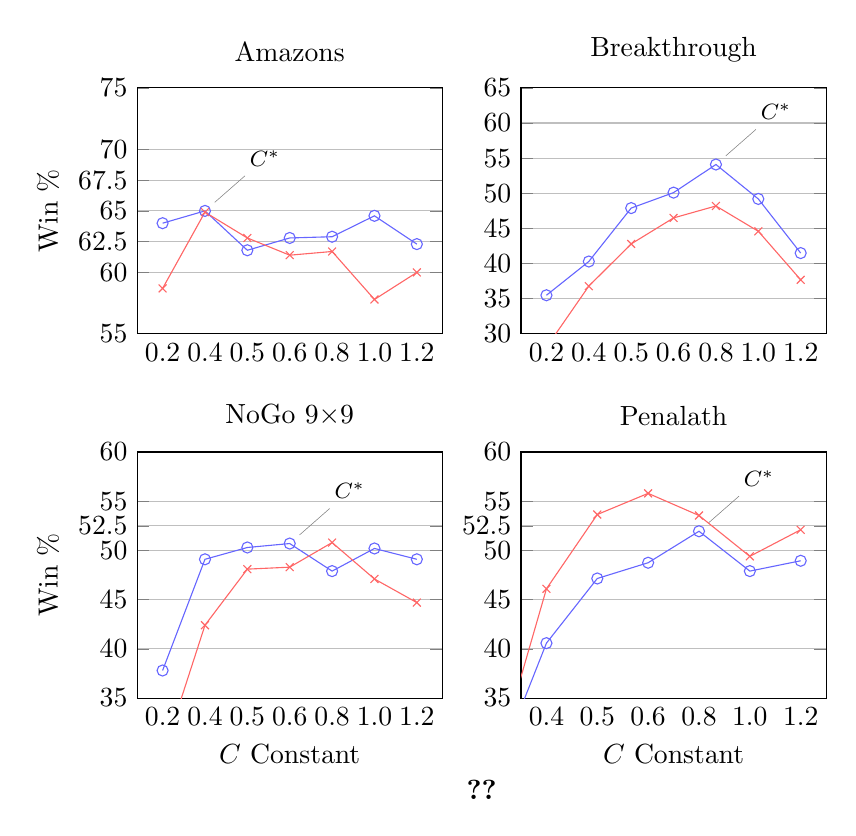
\begin{tikzpicture}
\begin{groupplot}
    [
        group style=
            {
            columns=2,
            rows=2,
            xlabels at=edge bottom,
            ylabels at=edge left,
            vertical sep= 1.5cm,
            },
        legend columns=2,
       	width  = 0.45*\textwidth,
        major x tick style = transparent,
        %ybar= 2 * \pgflinewidth,
        % bar width = 10pt,
        ymajorgrids = true,
        ylabel = {Win \%},
        xlabel= {$C$ Constant},
        symbolic x coords={0.2,0.4,0.5,0.6,0.8,1.0,1.2},
        xtick = data,
        ytick={0,20,40,50,60,70,80},
        scaled y ticks = false,
        enlarge x limits = 0.1,
        ymin=20,
        ymax=80,
    ]
% Amazons ----------------------------------------
\nextgroupplot[title=Amazons, ymin=55, ymax=75, ytick={55,60,62.5,65,67.5,70,75}]
\addplot[blue!60!white, mark=o]
	coordinates {
	(0.2,64) 
	(0.4,65)
	(0.5,61.8)
	(0.6,62.8)
	(0.8,62.9)
	(1.0,64.6)
	(1.2,62.3)};
\addplot[red!60!white, mark=x]
	coordinates {
	(0.2,58.7) 
	(0.4,64.9)
	(0.5,62.8)
	(0.6,61.4)
	(0.8,61.7)
	(1.0,57.8)
	(1.2,60.0)};
	\node at (axis cs:0.4,65) [pin=above right:{\smaller{$C^*$}}] {};
% Breakthrough -------------------------------------
\nextgroupplot[title=Breakthrough, ymin=30, ymax=65, ytick={20,30,35,40,45,50,55,60, 65}]
\addplot[blue!60!white, mark=o]
	coordinates {
	(0.2,35.5) 
	(0.4,40.3)
	(0.5,47.9)
	(0.6,50.1)
	(0.8,54.1)
	(1.0,49.2)
	(1.2,41.5)};
\addplot[red!60!white, mark=x]
	coordinates {
	(0.2,28.1) 
	(0.4,36.8)
	(0.5,42.8)
	(0.6,46.5)
	(0.8,48.2)
	(1.0,44.6)
	(1.2,37.7)};
	\node at (axis cs:0.8,54.1) [pin=above right:{\smaller{$C^*$}}] {};
% NoGo --------------------------------------------
\nextgroupplot[title=NoGo 9$\times$9, ymin=35, ymax=60, ytick={35,40,45,50,52.5,55,60}]
\addplot[blue!60!white, mark=o]
	coordinates {
	(0.2,37.80) 
	(0.4,49.10)
	(0.5,50.30)
	(0.6,50.70)
	(0.8,47.90)
	(1.0,50.20)
	(1.2,49.10)};
\addplot[red!60!white, mark=x]
	coordinates {
	(0.2,29.1) 
	(0.4,42.4)
	(0.5,48.10)
	(0.6,48.30)
	(0.8,50.80)
	(1.0,47.10)
	(1.2,44.70)};
\node at (axis cs:0.6,50.7) [pin=above right:{\smaller{$C^*$}}] {};
% Pentalath --------------------------------------------
\nextgroupplot[title=Penalath, legend to name=grouplegend3, ymin=35, ymax=60, ytick={35,40,45,50,52.5,55,60}]
\addplot[blue!60!white, mark=o]
	coordinates {
	(0.2,27.50) 
	(0.4,40.58)
	(0.5,47.15)
	(0.6,48.75)
	(0.8,51.95)
	(1.0,47.90)
	(1.2,48.95)};
	\addlegendentry{10,000 play-outs}
\addplot[red!60!white, mark=x]
	coordinates {
	(0.2,28.23) 
	(0.4,46.1)
	(0.5,53.65)
	(0.6,55.8)
	(0.8,53.55)
	(1.0,49.40)
	(1.2,52.10)};
	\addlegendentry{25,000 play-outs}
	\node at (axis cs:0.8,51.95) [pin=above right:{\smaller{$C^*$}}] {};
\end{groupplot}

    \node (legend) at ($(group c1r2.south)!0.5!(group c2r2.south)$)
      [below, yshift=-2\pgfkeysvalueof{/pgfplots/every axis title shift}]
      {\ref{grouplegend3}};

\end{tikzpicture}
     \caption[H-MCTS Solver with different $C$ values]{H-MCTS Solver vs. MCTS-Solver, varying values for H-MCTS' $C$ constant. \\ Win percentages with respect to H-MCTS. 1,000 games per data point.}
     \label{fig:h-mcts-s_v_mcts-s_uct_c}
\end{figure}



In Figure~\ref{fig:h-mcts-s_v_mcts-s_uct_c}, results are depicted for H-MCTS using different values for its $C$ constant. In each graph the constant previously tuned for UCT, $C^*$ is marked. Each game is played against MCTS-Solver using $C^*$ as the value for $C$.

The graphs show that for these games, the performance related to the $C$ values used by H-MCTS and UCT do not vary significantly. In Pentalath, H-MCTS' best measured value for $C$ differs from UCT's. It is likely that in Pentalath, H-MCTS benefits from an exploiting configuration of UCT, relying more on the values of nodes than their confidence bounds. This is possibly due to the extra exploration provided by Sequential Halving near the root, allowing fast exploitation on deeper plies.

Using the tuned $C=0.6$ constant found for Pentalath, three additional experiments were performed to determine the influence of the tuned parameter. The results of these experiments are presented in Table~\ref{tab:uct-s_hmcts-s_C_pent}, compared to the results presented in Table~\ref{tab:uct-s_hmcts-s}, in the 25,000 case H-MCTS' performance apparently increased by up to 2.2\%, which is not a significant improvement over the previous results.

\begin{table}[hb]
\centering
\captionsetup{justification=centering}
\tabcolsep=0.3cm
\scalebox{1.0}{
\begin{tabular}{rllll}
\hline
\multicolumn{2}{c|}{} & \multicolumn{1}{c}{\textbf{10,000}} & \multicolumn{1}{c}{\textbf{25,000}} & \multicolumn{1}{c}{\textbf{50,000}}\\ 
\textbf{Game} & \multicolumn{1}{c|}{\textbf{$B$}} & \multicolumn{1}{c}{\textbf{play-outs}} & \multicolumn{1}{c}{\textbf{play-outs}} & \multicolumn{1}{c}{\textbf{play-outs}} \\ [1mm] 
\cline{1-5}
\multicolumn{2}{c|}{} \\ [-3mm]
Pentalath &\multicolumn{1}{l|}{90}	& 48.6 $\pm$ 2.2	& {\bf{55.7}} $\pm$ 2.2 & 	{\bf{55.6}} $\pm$ 2.2			\\ [.5mm] 
\hline
\end{tabular}
}
\vspace{3mm}
{\caption[H-MCTS Solver vs. MCTS-Solver, tuned $C$]{H-MCTS Solver vs. MCTS-Solver, tuned $C$ for H-MCTS: $C=0.6$, and UCT: $C=0.8$.\\ Win percentages with respect to H-MCTS, 2,000 games.} \label{tab:uct-s_hmcts-s_C_pent}}
\end{table}

\begin{figure}[ht]
\centering
\captionsetup{justification=centering,margin=1cm}
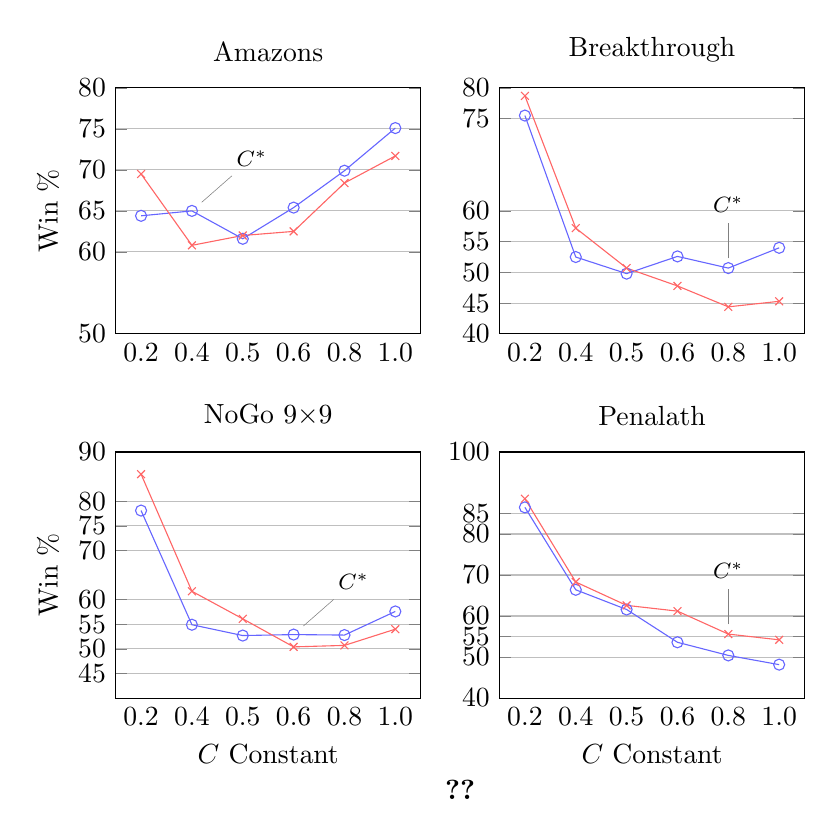
\begin{tikzpicture}
\begin{groupplot}
    [
        group style=
            {
            columns=2,
            rows=2,
            xlabels at=edge bottom,
            ylabels at=edge left,
            vertical sep= 1.5cm,
            },
        legend columns=2,
       	width  = 0.45*\textwidth,
        major x tick style = transparent,
        %ybar= 2 * \pgflinewidth,
        % bar width = 10pt,
        ymajorgrids = true,
        ylabel = {Win \%},
        xlabel= {$C$ Constant},
        symbolic x coords={0.2,0.4,0.5,0.6,0.8,1.0,1.2},
        xtick = data,
        ytick={0,20,40,50,60,70,80},
        scaled y ticks = false,
        enlarge x limits = 0.1,
        ymin=20,
        ymax=80,
    ]
% Amazons ----------------------------------------
\nextgroupplot[title=Amazons, ymin=50, ymax=80, ytick={50,60,65,70,75, 80}]
\addplot[blue!60!white, mark=o]
	coordinates {
	(0.2,64.4) 
	(0.4,65)
	(0.5,61.6)
	(0.6,65.4)
	(0.8,69.9)
	(1.0,75.1)};
\addplot[red!60!white, mark=x]
	coordinates {
	(0.2,69.5) 
	(0.4,60.8)
	(0.5,62.0)
	(0.6,62.5)
	(0.8,68.4)
	(1.0,71.7)};
	\node at (axis cs:0.4,65) [pin=above right:{\smaller{$C^*$}}] {};
% Breakthrough -------------------------------------
\nextgroupplot[title=Breakthrough, ymin=40, ymax=80, ytick={20,30,35,40,45,50,55,60,75,80}]
\addplot[blue!60!white, mark=o]
	coordinates {
	(0.2,75.5) 
	(0.4,52.5)
	(0.5,49.8)
	(0.6,52.6)
	(0.8,50.7)
	(1.0,54.0)};
\addplot[red!60!white, mark=x]
	coordinates {
	(0.2,78.7) 
	(0.4,57.2)
	(0.5,50.7)
	(0.6,47.8)
	(0.8,44.4)
	(1.0,45.3)};
	\node at (axis cs:0.8,50.7) [pin=above:{\smaller{$C^*$}}] {};
% NoGo --------------------------------------------
\nextgroupplot[title=NoGo 9$\times$9, ymin=40, ymax=90, ytick={45,50,55,60,70,75,80,90}]
\addplot[blue!60!white, mark=o]
	coordinates {
	(0.2,78.10) 
	(0.4,54.90)
	(0.5,52.70)
	(0.6,52.90)
	(0.8,52.80)
	(1.0,57.60)};
\addplot[red!60!white, mark=x]
	coordinates {
	(0.2,85.50) 
	(0.4,61.70)
	(0.5,56.10)
	(0.6,50.40)
	(0.8,50.70)
	(1.0,54.0)};
\node at (axis cs:0.6,52.9) [pin=above right:{\smaller{$C^*$}}] {};
% Pentalath --------------------------------------------
\nextgroupplot[title=Penalath, legend to name=grouplegend4, ymin=40, ymax=100, ytick={40,50,55,60, 70, 80,85,100}]
\addplot[blue!60!white, mark=o]
	coordinates {
	(0.2,86.5) 
	(0.4,66.4)
	(0.5,61.6)
	(0.6,53.6)
	(0.8,50.4)
	(1.0,48.15)};
	\addlegendentry{10,000 play-outs}
\addplot[red!60!white, mark=x]
	coordinates {
	(0.2,88.6) 
	(0.4,68.3)
	(0.5,62.6)
	(0.6,61.2)
	(0.8,55.6)
	(1.0,54.2)};
	\addlegendentry{25,000 play-outs}
	\node at (axis cs:0.8,55.6) [pin=above:{\smaller{$C^*$}}] {};
\end{groupplot}

    \node (legend) at ($(group c1r2.south)!0.5!(group c2r2.south)$)
      [below, yshift=-2\pgfkeysvalueof{/pgfplots/every axis title shift}]
      {\ref{grouplegend4}};

\end{tikzpicture}
     \caption[H-MCTS and UCT with suboptimal $C$ values]{H-MCTS Solver vs. MCTS-Solver using the same UCT $C$ constant. \\ Win percentages with respect to H-MCTS. 1,000 games per data point.}
     \label{fig:h-mcts-s_v_mcts-s_uct_subopt_c}
\end{figure}



Because H-MCTS is less dependent on the $C$ constant for its exploration than UCT, it is likely that when a non-optimal value is used for $C$, it has a smaller effect on H-MCTS' performance than it has for UCT's. To determine whether this holds, an experiment was performed in which both H-MCTS and UCT use the same, but varying $C$ constants. This experiment aims to show whether H-MCTS is more stable with respect to the $C$ constant than UCT. 

Figure~\ref{fig:h-mcts-s_v_mcts-s_uct_subopt_c} shows the results of this experiment. In each graph, the constant previously optimized $C^*$ is marked. In every domain tested, when both H-MCTS and UCT use a non-optimal $C$ constant, H-MCTS significantly outperforms UCT in distinct cases. Using a low constant such as 0.2 or 0.4, which means UCT will exploit promising moves faster, H-MCTS significantly outperforms UCT in all cases. When a higher than optimal value is used this increase in performance is only visible in Amazons and NoGo. In Pentalath and Breakthrough a value for $C$ which is too high is in some cases better handled by UCT.

This result is important in domains such as General Game Playing (GGP), because in GGP agents have no prior knowledge of the games being played. As such, the UCT constant cannot be optimally tuned for each game in GGP competitions. Using H-MCTS with an approximate value for $B$ possibly circumvents this problem, because it is less sensitive to suboptimal values for $C$.

% ------------------------------------------------------------------
% ------------------- ::::::: Conclusion ::::::: -------------------
% ------------------------------------------------------------------
\chapter{Conclusion}
\label{chap:conclusion}
\begin{chaptercontents}
Reflecting on the research questions and problem statement, conclusions are drawn. Moreover, possible directions for future research are provided.
\end{chaptercontents}

\section{Research Questions}
In this section the findings presented in this thesis are related to the research questions proposed in Chapter~\ref{chap:intro}.

\vspace{2mm}
\textbf{Research question 1:} How can a search technique minimize both simple, and cumulative regret in a game tree?
\vspace{2mm}

In Chapter~\ref{chap:mab} the main findings of the research performed be~\citeaby{Bubeck11Pure} were laid out in order to form the basis for minimizing both types of regret in a single tree. Concluding that cumulative and simple regret share conflicting bounds, and that no single selection policy can efficiently minimize both types of regret. Therefore, a combination of selection policies is required when minimizing both types of regret. Moreover, Chapter~\ref{chap:mab} discusses two recently introduced methods whit low bounds on simple regret in multi-armed bandits, Successive Rejects and Sequential Halving. Both are potential candidates to use as a selection policy in MCTS. In Chapter~\ref{chap:mctssr}, research into two state-of-the art MCTS techniques based on simple regret was discussed. The scheme presented by~\citeaby{tolpin2012mcts} gives the inspiration for minimizing simple regret only near the root. Moreover, a more recent algorithm SHOT~\citebay{Cazenave14SHOT} was shown to improve performance in games. SHOT uses Sequential Halving as its selection policy, and is therefore a suitable candidate to minimize simple regret in MCTS. The two methods discussed in Chapter~\ref{chap:mctssr} were combined in Chapter~\ref{chap:hybmcts}, in which a new technique, Hybrid MCTS (H-MCTS) was proposed, which combines SHOT and UCT in a single tree.

H-MCTS uses SHOT near the root, and UCT when overall budget is low, and therefore benefits from both the low simple regret offered by Sequential Halving, and the fast convergence and any time property of UCT. Consequently, the search tree is composed of a \emph{simple regret tree} at the root, and \emph{UCT trees} rooted at the leafs of the simple regret tree.

\vspace{2mm}
\textbf{Research question 2:} When should selection switch from simple to cumulative regret minimization in the tree?
\vspace{2mm}

\citeaby{Bubeck11Pure} showed that only when given a sufficiently large budget, should simple regret minimization be preferred over UCT. Therefore, whenever a Sequential Halving round can be initiated with a budget per child higher than $B$, we continue in the simple regret tree. Otherwise the budget is assigned to UCT, which runs $b$ simulations, and returns the result of their play-outs. Based on the available budget, H-MCTS' simple regret tree can expand deeper to provide better bounds on simple regret on the best-replies of rooted subtrees. 

In Chapter~\ref{chap:experiments} results for different values of $B$ are shown for Amazons, Breakthrough, NoGo and Pentalath. In most cases the tuned value remains stable when the number of allocated play-outs increases.

\vspace{2mm}
\textbf{Research question 3:} Do pure exploration selection policies in H-MCTS improve performance in two-player games?
\vspace{2mm}

H-MCTS uses Sequential Halving as its simple regret minimizing selection policy. To answer this question, experiments were performed, of which the results are presented in Chapter~\ref{chap:experiments}. H-MCTS' performance is assessed in six distinct two-player games. Although performance did not increase in all experimental cases, H-MCTS was able to boost performance considerably in several experiments. In Amazons and Pentalath H-MCTS gave a significant boost to performance. When using an informed play-out in Breakthrough, H-MCTS outperformed UCT given a sufficient budget. Moreover, with a fixed-budget H-MCTS outperformed SHOT in 10 out of 12 cases, it consistently outperformed SHOT given a budget of 25,000 play-outs.

\begin{itemize}

\item In \emph{Amazons}, likely due to its high branching factor, H-MCTS increases performance by up to 64.9\%. In all cases tested did H-MCTS improve performance over UCT. With a budget of 25,000 play-outs, H-MCTS performed significantly better against SHOT with a budget of 25,000 play-outs.

\item In \emph{AtariGo}, H-MCTS outperformed UCT with 69.1\% given a budget of 25,000 play-outs. Moreover, H-MCTS won up to 61.3\% of the games against SHOT.

\item In \emph{Ataxx}, H-MCTS performed better than UCT and SHOT in all experiments. H-MCTS outperformed UCT up to 65.2\%.

\item In \emph{Breakthrough}, H-MCTS outperforms UCT consistently up to 61.3\% when an informed play-out policy is used.

\item In \emph{NoGo}, the performance of H-MCTS is on-par with UCT. In none of the experiments did H-MCTS improve performance in this domain over UCT. However, against SHOT, H-MCTS performs better in all cases.

\item In \emph{Pentalath} performance increased up to 55.7\% for H-MCTS with the solver enabled. In this domain, the tuned $B$ constant was stable for budgets of both 10,000, 25,000, and 50,000 play-outs. Moreover, performance increased with the total budget assigned. In a time-based experiment H-MCTS outperformed UCT significantly, by 60.7\%.
\end{itemize} 

Finally, because H-MCTS is less sensitive to the value of UCT's $C$ constant used by UCT, the technique consistently outperforms UCT whenever both algorithms use a suboptimal value for $C$.

\vspace{2mm}
\textbf{Research question 4:} How can the MCTS-Solver be adapted to work with SHOT and H-MCTS?
\vspace{2mm}

The H-MCTS Solver was adapted to SHOT to be used in H-MCTS, where is is combined with the MCTS-Solver~\citebay{Winands2008} in the UCT tree, the new technique is named H-MCTS Solver. H-MCTS Solver ensures that the subset of children selected by Sequential Halving remains valid, and redistributes all unspent budget whenever a solved node is encountered. Moreover, it handles the interconnection between the simple regret and UCT trees when UCT returns the result of a solved position.

The implementation of the solver was validated by comparing UCT, H-MCTS and SHOT against their counterparts with the respective solver enabled. It was shown to be a highly beneficial enhancement in SHOT in the game Pentalath, and to a lesser extent in Breakthrough. However, in most experiments with H-MCTS Solver, it performed on par when playing against itself with a disabled solver. This may be due to the domains chosen for experimentation, as the same experiment with the MCTS-Solver showed similar results. It is possible that in less tactical domains with fewer traps the solver has a higher impact.

H-MCTS Solver was shown to outperform MCTS-Solver in different cases. In Breakthrough, when using a heuristic play-out policy, H-MCTS Solver won up to 61.3\% against MCTS-Solver. Moreover, in Pentalath the beneficial performance of H-MCTS Solver against MCTS-Solver increased from 50.8\% to 55.7\% given budgets of 10,000 up to 50,000 play-outs, respectively. Both cases show that there is a benefit of using the solver in H-MCTS when competing with UCT.
\newpage
\section{Problem Statement}

\vspace{2mm}
\textbf{Problem statement:} How can a Monte-Carlo Tree Search variant be constructed to minimize both simple, and cumulative regret effectively?
\vspace{2mm}

In this thesis an MCTS technique is presented based on the results of research in regret theory. The main findings of research performed by~\citeaby{Bubeck11Pure} were adapted into the form of a Hybrid MCTS technique (H-MCTS). Based on minimizing simple regret near the root, where the overall budget is high, and cumulative regret deeper in the tree~\citebay{tolpin2012mcts}. Based on available budget H-MCTS' simple regret tree can expand deeper to provide better bounds on simple regret on the best-replies of subtrees of the simple regret tree. The simple regret tree is traversed in a similar manner as SHOT~\citebay{Cazenave14SHOT}, and when a certain budget threshold $B$ is reached, selection switches to UCT. A number of play-outs are assigned to to the selected UCT tree, and the total result of these are back-propagated to the simple regret tree.

Results show that in different two-player games, H-MCTS performs either better than, or on par with UCT. In Amazons, Ataxx, and AtariGo, H-MCTS outperforms UCT by up to 69.1\%. Moreover, H-MCTS performed better than SHOT given the same allocation of play-outs in 10 out of 12 experiments performed. However, in $9\times 9$ NoGo no significant performance increase was shown against UCT. H-MCTS was shown to provide stable results in Pentalath, given an increasing budget of play-outs H-MCTS' performance significantly increased over UCT. In Pentalath, H-MCTS Solver outperformed MCTS-Solver up to 55.7\% given a play-out budget of 50,000. Moreover, results in Breakthrough give evidence that when a heuristic play-out policy is used, H-MCTS outperforms MCTS, both with the solver enabled and disabled. In the experiment presented, H-MCTS Solver won up to 61.3\% against MCTS-Solver in Breakthrough with a heuristic play-out policy for both players.

H-MCTS was shown to be faster than UCT in terms of the number of simulations per second. This resulted in an increased performance in several cases, but most notably in Pentalath, where H-MCTS won up to 60.7\% of the games when given the same deliberation time as UCT. In Pentalath, H-MCTS was approximately 7\% faster than UCT. In Breakthrough, with heuristic play-outs, H-MCTS was approximately 4\% faster than UCT. However, no significant performance improvements were achieved due to this increase in speed in Breakthrough.

The Upper/Lower Bounds enhancement was shown not to benefit performance over standard H-MCTS. This gives evidence that the increased exploration near the root performed by H-MCTS is the beneficial factor to the increased performance shown in the other experiments. When unpromising moves are removed from selection too early, the benefit of using the Sequential Halving selection policy declines.

Finally, experiments were performed to determine the robustness of H-MCTS with respect to the $C$ constant used by UCT. The first experiment determined that in Pentalath $C=0.6$ performed better than the previously optimized value for UCT, in all other games, the best used value for the constant did not change. The second experiment showed that H-MCTS outperforms UCT in most cases when both techniques use a suboptimal $C$ constant. This result is important in the General Game Playing (GGP) domain. Generally, the $C$ constant is tuned by experimentation per game. However, in GGP the agent does not know beforehand which game it is playing, and therefore the value used for $C$ is likely suboptimal. H-MCTS outperforms UCT when using a suboptimal value for the $C$ constant, and therefore may improve results in GGP.

\section{Future Research}

Although the hybrid technique is founded on theoretical work in both multi-armed bandits, and MCTS, it was not proven that it provides better bounds on simple regret when compared to UCT. This is work for future research. In order to show that H-MCTS exhibits lower simple regret in practice, the technique should be validated in smaller, proven games for which the game-theoretic value of each action is known. 

H-MCTS outperformed UCT in several cases, which leads to the following new research questions, open for future research:
\begin{enumerate}
\item In Amazons, likely due to its high branching factor, H-MCTS increases performance by up to 64.9\%. More research into domains with such large branching factors may show similar benefits.
\item In Breakthrough, the performance benefit of H-MCTS increased drastically when informed play-outs were enabled. Although this was only shown in Breakthrough in this thesis, it is possible that a heuristically improved engine may benefit from H-MCTS.
\item The optimal $C$ constant to be used in H-MCTS was shown to differ from UCT in several cases. The cause of this difference, and how both the $C$ and $B$ constants interact remains open to future research.
\item In this thesis H-MCTS is presented as a combination of SHOT and UCT. However, it is possible that other selection policies in the simple regret tree offer better performance in specific domains. How the performance of H-MCTS is influenced in different domains by using, for instance Successive Rejects, in the simple regret tree remains an open research question.
\item H-MCTS outperforms UCT when using a suboptimal value for the $C$ constant, and therefore may improve results in GGP. Further research in using H-MCTS for GGP may result in improved results in this domain.
\end{enumerate}

The speed benefits of H-MCTS, combined with parallelization of the algorithm is open to investigation. H-MCTS can be parallelized efficiently by dividing budgets in the simple regret tree over multiple threads~\citebay{Cazenave14SHOT}.

An open research direction relates to back-propagation in MCTS in general. Using UCT, the results of play-outs are back-propagated and averaged throughout the tree. This averaging is possible because, over time UCT tends to select the best node exclusively. However, when using a pure exploration policy, this is not the case, and back-propagated results do not tend toward a best-reply. A different back-propagation strategy may achieve better results when using for instance Sequential Halving as a selection policy.

Finally, in this thesis H-MCTS' switching point between selection policies is determined by a tuned constant $B$. However, alternative methods may be used to tune the switching point. For instance a fixed depth could be used or a time-constraint. Further investigation is required to find methods to determine when to change selection from cumulative to simple regret minimization.

\bibliography{thesis} \emptypage

\end{document}
